\documentclass[journal]{IEEEtran}

\usepackage{amsmath}
\usepackage{amsfonts}
\usepackage{gensymb}
\usepackage{graphicx}
\usepackage{float}
\usepackage[small,bf]{caption}
\usepackage{subcaption}
\usepackage{url}
\usepackage{color}
\usepackage{epstopdf}
\usepackage{cuted}
\usepackage{tikz}
\usepackage{tabularx}
\usepackage{tabulary}
\usepackage{todonotes}
\usepackage{lipsum}
% \usepackage[caption=false]{subfig}

\usepackage[export]{adjustbox}


\graphicspath{{figures/},{pdf/},{eps/},{png/}}

\renewcommand{\Re}{\operatorname{\textbf{Re}}}
\renewcommand{\Im}{\operatorname{\textbf{Im}}}
\DeclareMathOperator{\Tr}{Tr}
\DeclareMathOperator{\argmin}{argmin}

\begin{document}

%%%%%%%%%%%%%%%%%%%%%%%%%%%%%%%%%%%%%%%%%%%%%%%%%%
%% TITLE
%%%%%%%%%%%%%%%%%%%%%%%%%%%%%%%%%%%%%%%%%%%%%%%%%%
% \title{JOURNAL - Optimal Phasor Tracking}
\title{Optimal Voltage Phasor Regulation for Switching Actions in Distribution Systems}

%%%%%%%%%%%%%%%%%%%%%%%%%%%%%%%%%%%%%%%%%%%%%%%%%%
%% AUTHORS
%%%%%%%%%%%%%%%%%%%%%%%%%%%%%%%%%%%%%%%%%%%%%%%%%%
\author{
\IEEEauthorblockN{Michael Sankur, Roel Dobbe,  Alexandra Von Meier, Emma M. Stewart, and Daniel B. Arnold}}
% \IEEEauthorblockA{*Department of Mechanical Engineering\\
% **Department of Electrical Engineering and Computer Science\\
% ***Energy and Resources Group\\
% University of California, Berkeley\\
% Berkeley, California 94720\\
% (dbarnold, msankur, dobbe, kwbrady, dcal, vonmeier) @berkeley.edu}}

\maketitle

%%%%%%%%%%%%%%%%%%%%%%%%%%%%%%%%%%%%%%%%%%%%%%%%%%
%% SPONSOR FOOTNOTE
%%%%%%%%%%%%%%%%%%%%%%%%%%%%%%%%%%%%%%%%%%%%%%%%%%
\let\thefootnote\relax\footnote{This work was supported in part by the U.S. Department of Energy ARPA-E program (DE-AR0000340), and the Department of Energy Office of Energy Efficiency and Renewable Energy under Contract No. DE-AC02-05CH11231.}

%%%%%%%%%%%%%%%%%%%%%%%%%%%%%%%%%%%%%%%%%%%%%%%%%%
%% ABSTRACT
%%%%%%%%%%%%%%%%%%%%%%%%%%%%%%%%%%%%%%%%%%%%%%%%%%
\begin{abstract}
\noindent The proliferation of Distributed Energy Resources (DER) presents both challenges and opportunities for utility operators to manage distribution systems more effectively.  Though it is desirable to use Optimal Power Flow (OPF) formulations to manage DER, such abstractions have historically required the use of semidefinite relaxations when modeling unbalanced distribution systems.  As it can be difficult to obtain tight relaxations when solving semidefinite OPFs, in this work we introduce an extension to a linear model of unbalanced power flow that is subsequently incorporated into an OPF formulation.  We then apply this OPF to control the real and reactive power output of DER to minimize voltage phasor differences across switches, while maintaining proper voltage magnitudes throughout the feeder.  In so doing, we ensure that large amounts of power will not be instantaneously transferred as a result of switching actions.  Simulation results confirm the ability of the OPF to simultaneously minimize voltage phasor differences and regulate system voltage magnitudes.
\end{abstract}

%%%%%%%%%%%%%%%%%%%%%%%%%%%%%%%%%%%%%%%%%%%%%%%%%%
%% IEEE KEYWORDS
%%%%%%%%%%%%%%%%%%%%%%%%%%%%%%%%%%%%%%%%%%%%%%%%%%
% \begin{IEEEkeywords}
% Distributed energy resources, Voltage regulation,  Load Following, Model Predictive Control, Distributed Plug Load Control, Battery Storage Optimization
% \end{IEEEkeywords}

% \section*{Nomenclature}

% \noindent $n$ : Number of nodes along feeder \\
\noindent $V_{\phi,k}$ : Voltage phasor at node $k$ on phase $\phi$ \\
\noindent $\mathbb{V}_{k}$ : Vector of voltage phasors at node $k$ \\
\noindent $y_{\phi,k}$ : Square magnitude of voltage at node $k$ on phase $\phi$ \\ %s.t. $Y_{\phi,k} = \left| V_{\phi,k} \right| ^2$ \\
\noindent $\mathbb{Y}_{k}$ : Vector of square magnitudes of voltage at node $k$ \\
\noindent $Z_{\phi \phi,jk}$ : Impedance of segment $(j,k)$ on phase $\phi$ \\
\noindent $Z_{\phi \psi,jk}$ : Impedance of segment $(j,k)$ between phases ($\phi,\psi$) \\
\noindent $\mathbb{Z}_{jk}$ : Impedance matrix of line segment $(j,k)$ \\
\noindent $I_{\phi,k}$ : Current phasor entering node $k$ on phase $\phi$ \\
\noindent $\mathbb{I}_{k}$ : Vector of current phasors entering node $k$ \\
\noindent $i_{\phi,k}$ : Load current of phase $\phi$ at node $k$ \\
\noindent $\mathbf{i}_{k}$ : Vector of load currents at node $k$ \\
\noindent $S_{\phi,k}$ : Phasor of complex power entering node $k$ on phase $\phi$ \\
\noindent $\mathbb{S}_{k}$ : Vector of complex power phasors entering node $k$ \\
\noindent $s_{\phi,k}$ : Complex load on phase $\phi$ at node $k$ \\
\noindent $\mathbf{s}_{k}$ : Vector of complex loads at node $k$ \\
\noindent $u_{\phi,k}$ : Inverter VAR dispatch on phase $\phi$ at node $k$

\section{Introduction}

Coordination of a diverse set of Distributed Energy Resources (DER) presents many challenges to utility operators, who strive to ensure power of sufficient quality and quantity is available to retail customers at least cost.  Such assets can vary in size from residential rooftop PV units to larger PV arrays and, perhaps, battery storage systems located at residential, commercials and industrial sites.  As has been experienced in Hawaii~\cite{stewart2013analysis}, the negative impact of high levels of distributed PV under current interconnection standards is significant, and has led to financial impacts to both consumers and the utility.  However, distributed generation resources could, under the correct operational control scenarios, provide numerous benefits to the grid, including voltage support, VAR compensation, and ancillary services \cite{doe2015ADMS}.  

A variety of strategies for the management of DER presently exist for \emph{balanced} distribution system models.  Turitsyn et al. \cite{turitsyn2011options} considered a suite of distributed control strategies for reactive power compensation using four quadrant inverters.  The work of \cite{li2014real} studies distributed voltage regulation in the absence of communication, relying on locally obtained information.  In \cite{robbins2013two}, a two-stage control architecture for voltage regulation is considered where distributed controllers inject power based on local sensitivity measurements.  The authors of \cite{zhang2013local} study local voltage reference tracking with integral-type controllers, based on local voltage measurements.  The authors of \cite{farivar2011inverter} address voltage regulation and loss minimization through solving an Optimal Power Flow (OPF) problem, and address convexity issues using second order cone relaxations.  The work of \cite{lam2012optimal} also considers an OPF approach for voltage regulation in distribution networks by framing the decision-making process as a semidefinite program.  The authors provide conditions under which the semidefinite relaxation of the non-convex power flow problem is tight in balanced circuits. It is worth noting that many of the aforementioned approaches can be traced back to the seminal work of \cite{baran1989optimal}, that introduced nonlinear and linear-approximated recursive branch power flow models.

Approaches to coordinate DER in \emph{unbalanced} distribution systems, while being critical to the practical application in real distribution systems and microgrids \cite{doe2015ADMS}, are much less prevalent in the literature.  
While there is consensus about the physics-based models \cite{kersting2012distribution}, using these in an optimization setting is challenging. Perhaps the best known efforts have been put forth by Dall'Anese et. al \cite{dall2012optimization}, \cite{dall2013distributed}, who consider semidefinite relaxations for OPF problems in unbalanced systems, but do not provide conditions under which feasibility and optimality are guaranteed.  In addition to inefficient scaling as the problem size increases, the work of \cite{bitar2014} points out that it becomes more difficult to find a tight relaxation as the ratio of constraints to network buses increases.  A likely reason that more strategies focusing on coordination of distributed energy resources in unbalanced systems do not exist is the lack of suitable linear models that approximate three phase power flow. 

In our previous work \cite{arnold2015optimal}, we attempted to fill this void by proposing a linearized unbalanced power flow model that can be viewed as an extension of the \emph{LinDistFlow} \cite{baran1989optimal} linear approximation for balanced systems.  Using this linear model, we constructed an OPF formulation that dispatched reactive power resources from controllable DER to perform voltage balancing and regulation.  In this work, we extend the previously studied model; generalizing it to allow for other linearizations and comparing the results of OPF formulations that employ our linear model to those obtained via convex relaxations and semidefinite programming.

This work has three main contributions.  First, we derive a nonlinear model of unbalanced power flow in distribution systems which can be viewed as an extension of the \emph{DistFlow} system of equations, first studied in \cite{baran1989optimal}.  Secondly, we propose two approximations to linearize the model into a form suitable for incorporation into OPF formulations.  Finally, we evaluate the performance of the proposed linearizations numerically.  In one experiment, we demonstrate that an OPF driven by our linearized unbalanced power flow model produces results that closely approximate those obtained via an OPF that uses convex relaxations.  In a second experiment, we compare the proposed linearizations to perform voltage phase balancing and show that an iterative approach can be used to reduce linearization errors.

% Our results show that OPF formulations that utilize the linearized three phase \emph{LinDistFlow} model results in a dispatch of inverter VAR resources that successfully drives system voltages into acceptable regimes and simultaneously balances voltages by reducing magnitude differences between phases.

This work is organized as follows. A derivation of the three phase nonlinear power flow model is presented in Section \ref{sec:analysis}, along with two proposed linearization approaches.  Section \ref{sec:simulations} presents simulation results using the IEEE 13 node test feeder \cite{IEEEtestfeeder}.  Concluding remarks are provided in Section \ref{sec:conclusions}.  

% This section also introduces two linearizations for the derived model that render it suitable for incorporation into an OPF formulation.  In Section \ref{sec:simulation_results}, we formulate an OPF that uses one of the proposed linearization approaches to control DER to minimize feeder head real power consumption and compare these results to those obtained via solving a similiar OPF that uses convex relaxations and semidefinite programming.  Additionally, in this section, we formulate a second OPF designed to deploy DER resources to regulate and balance feeder voltages.  For this OPF, where it is not possible to formulate a representation as a semidefinite program, we compare the errors introduced by our proposed linearizations and discuss results from simulation.  Finally, concluding remarks are provided in Section \ref{sec:conclusion}.

\section{Analysis}
\label{sec:analysis}

 \subsection{Preliminaries}
 \label{subsec:preliminaries}

\renewcommand{\arraystretch}{1.15}
\setlength{\textfloatsep}{10pt}
\begin{table}[t]
\centering
\caption{NOMENCLATURE}
\begin{tabulary}{\textwidth}{LLL}
	\hline
	\hline
% $\mathcal{P}_{n}$ && Set of phases that exist at node $n$ \\
% \noindent $\mathcal{P}_{mn}$ & & Set of phases that exist on line $(m,n)$ \\
  \noindent $V_{n}^{\phi}$ & & Voltage phasor at node $n$ on phase $\phi$ \\
  \noindent $\mathbb{V}_{n}$ & & Vector of voltage phasors at node $n$ \\
  \noindent $y_{n}^{\phi}$ & & Square magnitude of voltage at node $n$ on phase $\phi$ \\
  \noindent $\mathbb{Y}_{n}$ & & Vector of square magnitudes of voltage at node $n$ \\
  $\theta_{n}^{\phi}$ & & Phase angle of voltage phasor at node $n$ on phase $\phi$ \\
  \noindent $Z_{mn}^{\phi \phi}$ & & Impedance of segment $(m,n)$ on phase $\phi$ \\
  \noindent $Z_{mn}^{\phi \psi}$ & & Impedance of segment $(m,n)$ between phases ($\phi,\psi$) \\
  \noindent $\mathbb{Z}_{mn}$ & & Impedance matrix of line segment $(m,n)$ \\
  \noindent $I_{n}^{\phi}$ & & Current phasor entering node $n$ on phase $\phi$ \\
  \noindent $\mathbb{I}_{n}$ & & Vector of current phasors entering node $n$ \\
  \noindent $i_{n}^{\phi}$ & & Load current of phase $\phi$ at node $n$ \\
  \noindent $\mathbf{i}_{n}$ & & Vector of load currents at node $n$ \\
  \noindent $S_{n}^{\phi}$ & & Phasor of complex power entering node $n$ on phase $\phi$ \\
  \noindent $\mathbb{S}_{n}$ & & Vector of complex power phasors entering node $n$ \\
  \noindent $s_{n}^{\phi}$ & & Complex load on phase $\phi$ at node $n$ \\
  \noindent $\mathbf{s}_{n}$ & & Vector of complex loads at node $n$ \\
%   \noindent $u_{n}^{\phi}$ & & Inverter real power dispatch on phase $\phi$ at node $n$ \\
%   \noindent $v_{n}^{\phi}$ & & Inverter VAR dispatch on phase $\phi$ at node $n$ \\
  \noindent $w_{n}^{\phi}$ & & Inverter complex dispatch on phase $\phi$ at node $n$ \\
  \noindent $\left( \cdot \right)^{*}$ & & Complex conjugate (transpose) of scalar (vector or matrix) \\
  \hline
  \hline
\end{tabulary}
\end{table}

Let $\mathcal{T} = (\mathcal{N}, \mathcal{E})$ denote a rooted tree graph representing an unbalanced radial distribution feeder, where $\mathcal{N}$ is the set of nodes of the feeder and $\mathcal{E}$ is the set of line segments. Nodes are indexed by $n = 0,1,\dots,N-1$, where $N$ is the order (number of nodes) of the distribution feeder, and node 0 denotes the feeder head (or substation). We treat node 0 as an infinite bus, decoupling interactions in the downstream distribution system from the rest of the grid. While the substation voltage may evolve over time, we assume this evolution takes place independently of DER control actions in $\mathcal{T}$. Each node and line segment can have up to three phases, labeled $a$, $b$, and $c$. For convenience, phases are referred to by the variables $\phi$ and $\psi$, where $\phi \in \{a,b,c \}$, $\psi \in \{a,b,c \}$. The current/voltage relationship between adjacent nodes $m$ and $n$ is captured by Kirchhoff's Voltage and Current Laws (KVL and KCL):
\begin{align}
	\begin{bmatrix}
		V_{m}^{a} \\
		V_{m}^{b} \\
		V_{m}^{c}
	\end{bmatrix}
	&=
	\begin{bmatrix}
		V_{n}^{a} \\
		V_{n}^{b} \\
		V_{n}^{c}
	\end{bmatrix}
	+
	\begin{bmatrix}
		Z^{aa}_{mn} & Z^{ab}_{mn} & Z^{ac}_{mn} \\
		Z^{ba}_{mn} & Z^{bb}_{mn} & Z^{bc}_{mn} \\
		Z^{ca}_{mn} & Z^{cb}_{mn} & Z^{cc}_{mn}
	\end{bmatrix}
	\begin{bmatrix}
		I_{n}^{a} \\
		I_{n}^{b} \\
		I_{n}^{c}
	\end{bmatrix} \label{eq:KVL}
% \end{align}
\\
% \begin{align}
\begin{bmatrix}
		I_{m}^{a} \\
		I_{m}^{b} \\
		I_{m}^{c}
	\end{bmatrix}
	&= \begin{bmatrix}
		i_{m}^{a} \\
		i_{m}^{b} \\
		i_{m}^{c}
	\end{bmatrix} + \sum_{n:(m,n) \in \mathcal{E}}
	\begin{bmatrix}
		I_{n}^{a} \\
		I_{n}^{b} \\
		I_{n}^{c}
	\end{bmatrix}\label{eq:KCL},
\end{align}
where $Z^{\phi \psi}_{mn} = r^{\phi \psi}_{mn} + jx^{\phi \psi}_{mn}$ (with $j = \sqrt{-1}$) denotes the complex impedance of line $(m,n)$ across phases $\phi$ and $\psi$. We assume  a complex load is served at each node, where the load on a phase $s_{n}^{\phi} = V_{n}^{\phi} {\left( i_{n}^{\phi} \right)}^{*} \in \mathbb{C}$ is defined as:
\begin{equation}
	s_{n}^{\phi} \left( V_{n}^{\phi} \right) = s_{n}^{\phi} \left(A_{PQ,n}^{\phi} + A_{Z,n}^{\phi} \left| V_{n}^{\phi} \right|^{2} \right) + w_{n}^{\phi}
    \label{eq:sV}
\end{equation}

\noindent where $A_{PQ,n}^{\phi} + A_{Z,n}^{\phi} = 1$, and $w_{n}^{\phi} = u_{n}^{\phi} + j v_{n}^{\phi}$ denotes the complex components of DER dispatch.
% \begin{equation}
% \begin{aligned}
% 	& s_{n}^{\phi} \left( V_{n}^{\phi} \right) = & & s_{n}^{\phi} \left(A_{PQ,n}^{\phi} + A_{I,n}^{\phi} \left| V_{n}^{\phi} \right| + A_{Z,n}^{\phi} \left| V_{n}^{\phi} \right|^{2} \right) \\
%     & & & - j h_{n}^{\phi} + w_{n}^{\phi}
%     \label{eq:sV}
% \end{aligned}
% \end{equation}
% \begin{equation}
% 	s_{n}^{\phi} \left( V_{n}^{\phi} \right) = s_{n}^{\phi} \left(A_{PQ,n}^{\phi} + A_{I,n}^{\phi} \left| V_{n}^{\phi} \right| + A_{Z,n}^{\phi} \left| V_{n}^{\phi} \right|^{2} \right) - j h_{n}^{\phi} + w_{n}^{\phi}
%     \label{eq:sV}
% \end{equation}


\subsection{Dist3Flow: Power and Losses}
\label{subsec:power}

For completness, we now present the derivation of the Dist3Flow power flow equations (see \cite{arnold2015model}, \cite{sankur2016linear}) between adjacent buses in an unbalanced distribution system. We begin with writing KVL for a line segment $(m,n)$ and KCL at a node $m$:
\begin{align}
	\mathbb{V}_{m} &= \mathbb{V}_{n} + \mathbb{Z}_{mn} \mathbb{I}_{n}
    \label{eq:KVL2}
    \\
    \mathbb{I}_{m} &= \mathbf{i}_{m} + \sum_{n:(m,n) \in \mathcal{E}} \mathbb{I}_{n}
    \label{eq:KCL2}
\end{align}

Right multiplying $\mathbb{V}_{m}$ by the complex conjugate transpose (denoted by $^*$) of Equation \eqref{eq:KCL2} and plugging in \eqref{eq:KVL2} on the RHS results in:
\begin{align}
	\mathbb{V}_{m} \mathbb{I}_{m}^{*} &= \mathbb{V}_{m}\mathbf{i}_{m}^{*} + \sum_{n:(m,n) \in \mathcal{E}} \mathbb{V}_{m} \mathbb{I}_{n}^{*} \nonumber \\
	&= \mathbb{V}_{m}  \mathbf{i}_{m}^{*} + \sum_{n:(m,n) \in \mathcal{E}} \mathbb{V}_{n}  \mathbb{I}_{n}^{*} + \mathbb{Z}_{mn} \mathbb{I}_{n} \mathbb{I}_{n}^{*} \label{eq:pow_11} \\
    &= \mathbb{V}_{m}  \mathbf{i}_{m}^{*} + \sum_{n:(m,n) \in \mathcal{E}} \mathbb{V}_{n}  \mathbb{I}_{n}^{*} + \mathcal L_{mn} \label{eq:pow_1},
\end{align}

\noindent where $\mathcal L_{mn} = \mathbb{Z}_{mn} \mathbb{I}_{n} \mathbb{I}_{n}^{*} \in \mathbb C^{3 \times 3}$ denotes the power loss matrix.

While \eqref{eq:pow_1} is a $3 \times 3$ matrix equation, we are only interested in the diagonal entries, which are the complex powers in each phase of the circuit.  We collect these entries into a $3 \times 1$ vector  equation, that yields a relation of the complex power flowing into node $m$ in terms of node $m$ demand, powers flowing into downstream nodes, and losses in downstream line segments:
\begin{equation}
	\mathbb{S}_{m} = \mathbf{s}_{m} + \sum_{n:(m,n) \in \mathcal{E}} \mathbb{S}_{n} + \mathbb{L}_{mn}
    \label{eq:pow_2}
\end{equation}

\noindent where $\mathbb{L}_{mn} \in \mathbb{C}^{3}$ and $\mathbb{L}_{mn}(i) = \mathcal L_{mn}(i,i)$ for $i = 1,2,3$. Eq. \eqref{eq:pow_2} is nonlinear and non-convex.  As in our previous works \cite{arnold2015optimal}, \cite{sankur2016linear} we introduce the following assumption:
\begin{description}
    \item[\textbf{A1:} ] $\mathbb{L}_{mn}$ is constant $\forall (m,n) \in \mathcal{E}$
\end{description}

\noindent Applying \textbf{A1} to \eqref{eq:pow_2} gives a linear equation for conservation of complex power, the \emph{LinDist3Flow} power equation. As in \cite{baran1989optimal}, we can further simplify this equation by selecting $\mathbb{L}_{mn} = {\left[0, \text{ } 0, \text{ } 0 \right]}^{T} \text{ } \forall (m,n) \in \mathcal{E}$, giving \eqref{eq:pow_2_lin}.
\begin{equation}
	\mathbb{S}_{m} \approx \mathbf{s}_{m} + \sum_{n:(m,n) \in \mathcal{E}} \mathbb{S}_{n}
    \label{eq:pow_2_lin}
\end{equation}

\subsection{Dist3Flow: Magnitude Equations}
\label{subsec:magnitude}

In this section, we present the derivation of the Dist3Flow voltage magnitude equations (see \cite{arnold2015model}, \cite{sankur2016linear}).  We do this to motivate the extension of the model to consider voltage angles in the following section, and to highlight a common structure shared between the voltage magnitude/complex power flow and voltage angle/complex power flow relationships. 

To start, we consider \eqref{eq:KVL2} on edge $(m,n) \in \mathcal{E}$ and right multiply both sides by their respective complex conjugate transpose, resulting in the $3 \times 3$ matrix equation:
\begin{align}
% \begin{aligned}
	\mathbb{V}_{m} \mathbb{V}_{m}^*  & =  \mathbb{V}_{n} \mathbb{V}_{n}^* + \mathbb{Z}_{mn} \mathbb{I}_{n} \mathbb{V}_{n}^* + \mathbb{V}_{n} \mathbb{I}_{n}^{*} \mathbb{Z}_{mn}^{*} + \mathbb{Z}_{mn} \mathbb{I}_{n} \mathbb{I}_{n}^{*} \mathbb{Z}_{mn}^{*} \nonumber \\
    & = \mathbb{V}_{n} \mathbb{V}_{n}^* + 2 \Re \left\{\mathbb{V}_{n} \mathbb{I}_{n}^{*} \mathbb{Z}_{mn}^{*} \right\} + \mathcal H_{mn},
\label{eq:mag_1}
% \end{aligned}
\end{align}

\noindent where $\mathcal H_{mn} = \mathbb{Z}_{mn} \mathbb{I}_{n} \mathbb{I}_{n}^{*} \mathbb{Z}_{mn}^{*} \in \mathbb C^{3 \times 3}$ denotes a matrix of higher order terms.  Noticing that for the scalar current ${\left( I^{\phi}_{n} \right)}^{*} = S_{n}^{\phi} {\left( V_{n}^{\phi} \right)}^{-1} \in \mathbb{C}$,  we can write \eqref{eq:mag_1} as:
\begin{equation}
	\begin{aligned}
		\mathbb{V}_{m} & \mathbb{V}_{m}^{*} = \mathbb{V}_{n} \mathbb{V}_{n}^{*} + \mathcal H_{mn} + \ldots \\
    	& \text{ } 2 \Re \left\{ \mathbb{V}_{n}
    	\begin{bmatrix}
    		S_{n}^{a} {\left( V_{n}^{a} \right)}^{-1} & S_{n}^{b} {\left( V_{n}^{b} \right)}^{-1} & S_{n}^{c} {\left( V_{n}^{c} \right)}^{-1}
    	\end{bmatrix}
%         \left[
%     		S_{n}^{a} {\left( V_{n}^{a} \right)}^{-1} \text{ } S_{n}^{b} {\left( V_{n}^{b} \right)}^{-1} \text{ } S_{n}^{c} {\left( V_{n}^{c} \right)}^{-1}
%     	\right]
    	\mathbb{Z}_{mn}^{*} \right\}.
    \end{aligned}
    \label{eq:mag_2}
\end{equation}

Now, we define $\gamma_{n}^{\phi \psi} = V_{n}^{\phi} {\left( V_{n}^{\psi} \right)}^{-1} \in \mathbb{C}$ as the ratio of voltages between phases $\phi$ and $\psi$ at node $n$, where $\phi,\psi \in \{ a,b,c \}$, and clearly $\gamma_{n}^{\phi \psi} = 1 $ if $\phi = \psi$. Applying this to \eqref{eq:mag_2} results in:
\begin{equation}
	\begin{aligned}
		\mathbb{V}_{m} & \mathbb{V}_{m}^{*} = \mathbb{V}_{n} \mathbb{V}_{n}^{*} + \mathcal H_{mn} + \ldots \\
    	& 2 \Re \left\{
    	\begin{bmatrix}
    		S_{n}^{a} & \gamma_{n}^{ab} S_{n}^{b} & \gamma_{n}^{ac} S_{n}^{c} \\
    		\gamma_{n}^{ba} S_{n}^{a} & S_{n}^{b} & \gamma_{n}^{bc} S_{n}^{c} \\
    		\gamma_{n}^{ca} S_{n}^{a} & \gamma_{n}^{cb} S_{n}^{b} & S_{n}^{c}
    	\end{bmatrix}
    	\mathbb{Z}_{mn}^* \right\} .
    \end{aligned}
    \label{eq:mag_4}
\end{equation}

We now gather the diagonal entries of \eqref{eq:mag_4} and place them into a $3 \times 1$ vector equation.  Defining the variable $y_{n}^{\phi} = | V_{n}^{\phi} |^{2}$, and the vector
$\mathbb{Y}_{n} = {\left[ y_{n}^{a}, \text{ } y_{n}^{b}, \text{ } y_{n}^{c} \right]}^{T}$
% $\mathbb{Y}_{n} = {\begin{bmatrix} y_{n}^{a} & y_{n}^{b} & y_{n}^{c} \end{bmatrix}}^{T}$
, \eqref{eq:mag_4} becomes:
\begin{align}
	& \mathbb{Y}_{m} = \mathbb{Y}_{n} + \mathbb{H}_{mn} + \ldots \nonumber \\
    & \text{ } 2 \Re \left\{
    \begin{bmatrix}
    	{\left( Z_{mn}^{aa} \right)}^{*} S_{n}^{a}  + \gamma_{n}^{ab} {\left( Z_{mn}^{ab} \right)}^{*} S_{n}^{b}  + \gamma_{n}^{ac} {\left( Z_{mn}^{ac} \right)}^{*} S_{n}^{c} \\
    	\gamma_{n}^{ba} {\left( Z_{mn}^{ba} \right)}^{*} S_{n}^{a} + {\left( Z_{mn}^{bb} \right)}^{*} S_{n}^{b} + \gamma_{n}^{bc} {\left( Z_{mn}^{bc} \right)}^{*} S_{n}^{c} \\
    	\gamma_{n}^{ca} {\left( Z_{mn}^{ca} \right)}^{*} S_{n}^{a} + \gamma_{n}^{cb} {\left( Z_{mn}^{cb} \right)}^{*} S_{n}^{b} + {\left( Z_{mn}^{cc} \right)}^{*} S_{n}^{c}
    \end{bmatrix}
	\right\}
    \label{eq:mag_5},
\end{align}

\noindent where $\mathbb{H}_{mn} \in \mathbb{C}^{3}$ and $\mathbb{H}_{mn}(i) = \mathcal H_{mn}(i,i)$ for $i = 1,2,3$.  Equation \eqref{eq:mag_5} can be restated by grouping the $\gamma$ and impedance terms into a $3\times 3$ matrix multiplied by a $3 \times 1$ vector of complex powers, which results in:
\begin{align}
	& \mathbb{Y}_{m} = \mathbb{Y}_{n} + \mathbb{H}_{mn} + \ldots \nonumber \\
    & \text{ } 2 \Re \left\{
    \begin{bmatrix}
    	{\left( Z_{mn}^{aa} \right)}^{*} & \gamma_{ab} {\left( Z_{mn}^{ab} \right)}^{*} & \gamma_{n}^{ab} {\left( Z_{mn}^{ac} \right)}^{*} \\
    	\gamma_{n}^{ba} {\left( Z_{mn}^{ba} \right)}^{*} & {\left( Z_{mn}^{bb} \right)}^{*} & \gamma_{n}^{ab} {\left( Z_{mn}^{bc} \right)}^{*} \\
    	\gamma_{n}^{ca} {\left( Z_{mn}^{ca} \right)}^{*} & \gamma_{n}^{cb} {\left( Z_{mn}^{cb} \right)}^{*} & {\left( Z_{mn}^{cc} \right)}^{*}
    \end{bmatrix}
    \begin{bmatrix}
    	S_{n}^{a} \\ S_{n}^{b} \\ S_{n}^{c}
    \end{bmatrix}
	\right\}
    \label{eq:mag_6}.
\end{align}

We can now rewrite \eqref{eq:mag_6} in terms of active and reactive components $\mathbb{P}_{n},\mathbb{Q}_{n} \in \mathbb C^{3}$:
\begin{equation}
	\mathbb{Y}_{m} = \mathbb{Y}_{n} + \mathbb{M}_{mn} \mathbb{P}_{n} + \mathbb{N}_{mn} \mathbb{Q}_{n} + \mathbb{H}_{mn},
    \label{eq:mag_7}
\end{equation}

\noindent where the elements of $\mathbb{M}_{mn}$ and $\mathbb{N}_{mn}$ are defined as:
\begin{align}
	\mathbb{M}_{mn} (\phi, \psi) &= 2\Re \left\{\gamma_{n}^{\phi \psi} {\left( Z_{mn}^{\phi \psi} \right)}^{*} \right\} \label{eq:mag_8} \\
    \mathbb{N}_{mn} (\phi, \psi) &= -2\Im \left\{\gamma_{n}^{\phi \psi} {\left( Z_{mn}^{\phi \psi} \right)}^{*} \right\} \label{eq:mag_9},
\end{align}

\noindent with $a=1$, $b=2$, and $c=3$ for indexing purposes on the LHS of \eqref{eq:mag_8} and \eqref{eq:mag_9} (e.g. $M_{mn}(a,b)$ refers to the (1,2) index so that $M_{mn} (1,2) = 2 \Re \{ \gamma_{n}^{ab} {\left( Z_{mn}^{ab} \right)}^{*} \}$). Finally, we express the $\gamma$ terms as generalized complex numbers, $\gamma_{n}^{\phi \psi} = \alpha_{n}^{\phi \psi} + j\beta_{n}^{\phi \psi} $,
%and organize \eqref{eq:mag_6} in terms of active and reactive components $\mathbb{P}_{n},\mathbb{Q}_{n} \in \mathbb C^{3}$:
and rewrite \eqref{eq:mag_8} and \eqref{eq:mag_9} as \eqref{eq:mag_10} and \eqref{eq:mag_11}, respectively:
\begin{align}
	\mathbb{M}_{mn} (\phi, \psi) &= 2\begin{cases}
    	 r_{mn}^{\phi \psi} &\mbox{if } \phi = \psi \\
         \alpha_{n}^{\phi \psi} r_{mn}^{\phi \psi} + \beta_{n}^{\phi \psi} x_{mn}^{\phi \psi} &\mbox{if } \phi \ne \psi
    \end{cases} \label{eq:mag_10}
\end{align}

\begin{align}
	\mathbb{N}_{mn} (\phi, \psi) &= 2\begin{cases}
    	 x_{mn}^{\phi \psi} &\mbox{if } \phi = \psi \\
         \alpha_{n}^{\phi \psi} x_{mn}^{\phi \psi} - \beta_{n}^{\phi \psi} r_{mn}^{\phi \psi} &\mbox{if } \phi \ne \psi
    \end{cases} \label{eq:mag_11}
\end{align}

% \noindent with $a=1$, $b=2$, and $c=3$ for indexing purposes on the LHS of \eqref{eq:mag_8} and \eqref{eq:mag_9} (e.g. $M_{mn}(a,b)$ refers to the (1,2) index).

% We notice that the entries of $\mathbb{M}_{mn}$ and $\mathbb{N}_{mn}$ can also be defined as following:
% \begin{align}
% 	\mathbb{M}_{mn} (\phi, \psi) &= 2\Re \left\{\gamma_{n}^{\phi \psi} {\left( Z_{mn}^{\phi \psi} \right)}^{*} \right\} \label{eq:mag_10} \\
%     \mathbb{N}_{mn} (\phi, \psi) &= -2\Im \left\{\gamma_{n}^{\phi \psi} {\left( Z_{mn}^{\phi \psi} \right)}^{*} \right\} \label{eq:mag_11},
% \end{align}

% \noindent where clearly $\gamma_{n}^{\phi \psi} = 1 \text{ } \forall n \in \mathcal{N}$ if $\phi = \psi$.

Eqs. \eqref{eq:mag_7} - \eqref{eq:mag_11} represent the portion of the \emph{Dist3Flow} equations that govern the relationship between squared voltage magnitudes between adjacent nodes and complex power flow.  This system, as it is nonlinear and nonconvex, is difficult to directly incorporate into an OPF formulation without the use of convex relaxations.  However, this system can be linearized via making the following assumptions:

\begin{description}
	\item[\textbf{A2:} ] $\mathbb{H}_{mn}$ is constant $\forall (m,n) \in \mathcal{E}$
	\item[\textbf{A3:} ] $\gamma_{n}^{\phi \psi}$ are constant $\forall n \in \mathcal{N}$, $\forall \phi \in \{a,b,c\}$, $\psi \in \{a,b,c\}$,  $\phi \ne \psi$    
\end{description}

% \noindent Assumption {A2} states that higher order terms are constant on all line segments $(m,n) \in \mathcal{E}$. Assumption {A3} states that voltage phasor ratios at all nodes are constant.
\noindent Application of assumptions \textbf{A2} and \textbf{A3} to the system of \eqref{eq:mag_7} - \eqref{eq:mag_11} results in a linear model that relates the squared magnitudes of nodal voltages and complex power flows to DER injected power.  We refer to the resulting system due to the application of \textbf{A2} and \textbf{A3} to \eqref{eq:mag_7} - \eqref{eq:mag_11} as the \emph{LinDist3Flow} magnitude equations.

The \emph{LinDist3Flow} magnitude equations can be further simplified via logical choices for the constant parameters of \textbf{A2} and \textbf{A3}.  Following the analysis presented in \cite{baran1989optimal}, we choose $\mathbb{H}_{mn} = {\left[0, \text{ } 0, \text{ } 0 \right]}^{T} \text{ } \forall (m,n) \in \mathcal{E}$.  Next we define the parameter $\sigma$ such that:
\begin{equation}
	\sigma = \frac{-1 + j\sqrt{3}}{2}, \quad \sigma^{2} = \frac{-1 - j\sqrt{3}}{2}
    \label{eq:sigma},
\end{equation}
\noindent and assign them to the $\gamma$ terms according to:
\begin{equation}
	\gamma_{n}^{ab} = \sigma \quad \gamma_{n}^{bc} = \sigma \quad \gamma_{n}^{ac} = \sigma^{2} \quad \forall n \in \mathcal{N}
    \label{eq:gamma}
\end{equation}

\noindent where clearly $\sigma = 1 \angle 120\degree$ and $\sigma^{2} = \sigma^{*}$.  This choice of parameters for \textbf{A3} reflects the ratio of nominal voltages at the distribution substation, where, typically, $V_{0}^{a} = 1\angle 0 \degree$, $V_{0}^{b} = 1\angle 240 \degree$, and $V_{0}^{c} = 1\angle 120 \degree$.  Choosing the $\gamma$ terms in this manner highlights the effect of the voltage ratio terms of \eqref{eq:mag_10} - \eqref{eq:mag_11} in rotating non-diagonal elements of the impedance matrix by $ \pm 120 \degree$.  With a bit of algebra, it is straightforward to verify that with these choices for \textbf{A2} and \textbf{A3}, Eqs. \eqref{eq:mag_7} - \eqref{eq:mag_11} become:
\begin{align}
	\mathbb{Y}_{m} &\approx \mathbb{Y}_{n} - \mathbb{M}_{mn} \mathbb{P}_{n} - \mathbb{N}_{mn} \mathbb{Q}_{n} \label{eq:mag_7_lin}
\end{align}
\begin{align}
	\mathbb{M}_{mn} &=
	\begin{bmatrix}
		-2 r_{mn}^{aa} & r_{mn}^{ab} - \sqrt{3} x_{mn}^{ab} & r_{mn}^{ac} + \sqrt{3} x_{mn}^{ac} \\
		r_{mn}^{ba} + \sqrt{3} x_{mn}^{ba} & -2 r_{mn}^{bb} & r_{mn}^{bc} - \sqrt{3} x_{mn}^{bc} \\
		r_{mn}^{ca} - \sqrt{3} x_{mn}^{ca} & r_{mn}^{cb} + \sqrt{3} x_{mn}^{cb} & -2 r_{mn}^{cc}
	\end{bmatrix} \label{eq:mag_8_lin}\\
	\mathbb{N}_{mn} &=
	\begin{bmatrix}
		-2 x_{mn}^{aa} & x_{mn}^{ab} + \sqrt{3} r_{mn}^{ab} & x_{mn}^{ac} - \sqrt{3} r_{mn}^{ac} \\
		x_{mn}^{ba} -\sqrt{3} r_{mn}^{ba} & -2 x_{mn}^{bb} & x_{bc} + \sqrt{3} r_{mn}^{bc}\\
		x_{mn}^{ca} + \sqrt{3} r_{mn}^{ca} & x_{mn}^{cb} -\sqrt{3} r_{mn}^{cb} & -2 x_{mn}^{cc}
	\end{bmatrix} \label{eq:mag_9_lin}.
\end{align}

The system of \eqref{eq:mag_7_lin} - \eqref{eq:mag_9_lin} was incorporated into an OPF formulation used to conduct simulations in this work (discussed in Section \ref{sec:simulation_results}). Notice that in the single phase case, this system reduces to a variant of the \emph{LinDistFlow} equations.


\subsection{Dist3Flow: Angle Equations}
\label{subsec:angle}

We now derive an extension of the \emph{Dist3Flow} system that relates differences in voltage angles between adjacent nodes to complex power flows.  This derivation shares many similarities with the analysis of Section \ref{subsec:magnitude}.  We start by multiplying the voltage at node $n$ by the complex conjugate of \eqref{eq:KVL2}:
\begin{equation}
	\mathbb{V}_{n} \mathbb{V}_{m}^* = \mathbb{V}_{n} \mathbb{V}_{n}^* + \mathbb{V}_{n} \mathbb{I}_{n}^{*} \mathbb{Z}_{mn}^{*}.
    \label{eq:angle_1}
\end{equation}

\noindent Using the definition of the scalar current $(I^{\phi}_{n})^* = S_{n}^{\phi} (V_{n}^{\phi})^{-1} \in \mathbb C$, \eqref{eq:angle_1} can be rewritten as:
\begin{equation}
\begin{aligned}
	\mathbb{V}_{n} & \mathbb{V}_{m}^* = \mathbb{V}_{n} \mathbb{V}_{n}^* + \ldots \\
    & \mathbb{V}_{n}
    \begin{bmatrix}
    	S_{n}^{a} {\left( V_{n}^{a} \right)}^{-1} &
        S_{n}^{b} {\left( V_{n}^{b} \right)}^{-1} &
        S_{n}^{c} {\left( V_{n}^{c} \right)}^{-1}
    \end{bmatrix} \mathbb{Z}_{mn}^{*}.
    \label{eq:angle_2}
\end{aligned}
\end{equation}

% \begin{align}
% 	\mathbb{V}_{n} & \mathbb{V}_{m}^* = \mathbb{V}_{n} \mathbb{V}_{n}^* + \ldots \nonumber \\
%     & \begin{bmatrix}
%     	S_{n}^{a} & V_{n}^{a} S_{n}^{b} (V_{n}^{b})^{-1} & V_{n}^{a} S_{n}^{c} (V_{n}^{c})^{-1} \\
%         V_{n}^{b} S_{n}^{a} (V_{n}^{a})^{-1} & S_{n}^{b} & V_{n}^{b} S_{n}^{c} (V_{n}^{c})^{-1} \\
%         V_{n}^{c} S_{n}^{a} (V_{n}^{a})^{-1} & V_{n}^{c} S_{n}^{b} (V_{n}^{b})^{-1} & S_{n}^{c}
%     \end{bmatrix} \mathbb{Z}_{mn}^{*}
%     \label{eq:angle_3}
% \end{align}

\noindent We substitute the previously defined $\gamma$ terms for $V_{n}^{\phi} {\left( V_{n}^{\psi} \right)}^{-1}$ to \eqref{eq:angle_2}, giving:
% As previously, $\gamma_{n}^{\phi , \psi}$  is defined as as the ratio of voltages between phases $\phi$ and $\psi$ at node $n$, or $\gamma_{n}^{\phi \psi} = V_{n}^{\phi} (V_{n}^{\psi})^{-1}$, where $\phi,\psi \in \{ a,b,c\}$ and $\phi \ne \psi$.  Applying this to \eqref{eq:angle_2} results in:
\begin{equation}
	\mathbb{V}_{n} \mathbb{V}_{m}^* = \mathbb{V}_{n} \mathbb{V}_{n}^* + \begin{bmatrix}
    	S_{n}^{a} & \gamma_{n}^{ab} S_{n}^{b} & \gamma_{n}^{ac} S_{n}^{c} \\
        \gamma_{n}^{ba} S_{n}^{a} & S_{n}^{b} & \gamma_{n}^{bc} S_{n}^{c} \\
        \gamma_{n}^{ca} S_{n}^{a} & \gamma_{n}^{cb} S_{n}^{b} & S_{n}^{c}
    \end{bmatrix} \mathbb{Z}_{mn}^{*}.
    \label{eq:angle_4}
\end{equation}

We now gather the diagonal entries of \eqref{eq:angle_4} and place them into a $3 \times 1$ vector equation. Here, we write the product of $V_{n}^{\phi}$ and $\left( V_{m}^{\phi} \right)^{*}$ in polar form, and apply the definition of $\mathbb{Y}_{n}$:
\begin{align}
	& \begin{bmatrix}
    	\left| V_{n}^{a} \right| \left| V_{m}^{a} \right| \angle \left( \theta_{n}^{a} - \theta_{m}^{a} \right) \\
        \left| V_{n}^{b} \right| \left| V_{m}^{b} \right| \angle \left( \theta_{n}^{b} - \theta_{m}^{b} \right) \\
        \left| V_{n}^{c} \right| \left| V_{m}^{c} \right| \angle \left( \theta_{n}^{c} - \theta_{m}^{c} \right)
    \end{bmatrix}
	= \mathbb{Y}_{n} + \ldots \nonumber \\
    & \quad
    \begin{bmatrix}
    	{\left( Z_{mn}^{aa} \right)}^{*} S_{n}^{a}  + \gamma_{n}^{ab} {\left( Z_{mn}^{ab} \right)}^{*} S_{n}^{b}  + \gamma_{n}^{ac} {\left( Z_{mn}^{ac} \right)}^{*} S_{n}^{c} \\
    	\gamma_{n}^{ba} {\left( Z_{mn}^{ba} \right)}^{*} S_{n}^{a} + {\left( Z_{mn}^{bb} \right)}^{*} S_{n}^{b} + \gamma_{n}^{bc} {\left( Z_{mn}^{bc} \right)}^{*} S_{n}^{c} \\
    	\gamma_{n}^{ca} {\left( Z_{mn}^{ca} \right)}^{*} S_{n}^{a} + \gamma_{n}^{cb} {\left( Z_{mn}^{cb} \right)}^{*} S_{n}^{b} + {\left( Z_{mn}^{cc} \right)}^{*} S_{n}^{c}
    \end{bmatrix}
    \label{eq:angle_5}
\end{align}

The left hand side of \eqref{eq:angle_5} can be separated into its real and imaginary parts as $\angle \left( \theta_{n}^{\phi} - \theta_{m}^{\phi} \right) = \cos \left( \theta_{n}^{\phi} - \theta_{m}^{\phi} \right) + j \sin \left( \theta_{n}^{\phi} - \theta_{m}^{\phi} \right) $. Taking the imaginary part of \eqref{eq:angle_5} and separating the RHS into a matrix of rotated impedance terms multiplying a vector of power at node $n$ results in \eqref{eq:angle_6}:
\begin{align}
	& \begin{bmatrix}
    	\left| V_{n}^{a} \right| \left| V_{m}^{a} \right| \sin \left( \theta_{n}^{a} - \theta_{m}^{a} \right) \\
        \left| V_{n}^{b} \right| \left| V_{m}^{b} \right| \sin \left( \theta_{n}^{b} - \theta_{m}^{b} \right) \\
        \left| V_{n}^{c} \right| \left| V_{m}^{c} \right| \sin \left( \theta_{n}^{c} - \theta_{m}^{c} \right)
    \end{bmatrix}
	= \ldots \nonumber \\
    & \quad \Im \left\{
    \begin{bmatrix}
    	{\left( Z_{mn}^{aa} \right)}^{*} & \gamma_{n}^{ab} {\left( Z_{mn}^{ab} \right)}^{*} & \gamma_{n}^{ac} {\left( Z_{mn}^{ac} \right)}^{*} \\
        \gamma_{n}^{ba} {\left( Z_{mn}^{ba} \right)}^{*} & {\left( Z_{mn}^{bb} \right)}^{*} & \gamma_{n}^{bc} {\left( Z_{mn}^{bc} \right)}^{*} \\
        \gamma_{n}^{ca} {\left( Z_{mn}^{ca} \right)}^{*} & \gamma_{n}^{cb} {\left( Z_{mn}^{cb} \right)}^{*} & {\left( Z_{mn}^{cc} \right)}^{*}
    \end{bmatrix}
    \begin{bmatrix}
    	S_{n}^{a} \\
        S_{n}^{b} \\
        S_{n}^{c}
    \end{bmatrix}
    \right\}
    \label{eq:angle_6}.
\end{align}

We now follow the same steps taken to taken to transform \eqref{eq:mag_6} into \eqref{eq:mag_7} - \eqref{eq:mag_11}, and rewrite \eqref{eq:angle_6} in terms of active and reactive power components $\mathbb{P}_{n},\mathbb{Q}_{n} \in \mathbb C^{3}$:
% Expressing $\gamma_{n}^{\phi \psi}$ as a general complex number $\gamma_{n}^{\phi \psi} = \alpha_{n}^{\phi \psi} + j \beta_{n}^{\phi \psi}$, we can rewrite \eqref{eq:angle_6} in in terms of active and reactive components $\mathbb{P}_{n},\mathbb{Q}_{n} \in \mathbb C^{3}$:
% \begin{equation}
%   \begin{bmatrix}
%           \left| V_{n}^{a} \right| \left| V_{m}^{a} \right| \sin \left( \theta_{n}^{a} - \theta_{m}^{a} \right) \\
%           \left| V_{n}^{b} \right| \left| V_{m}^{b} \right| \sin \left( \theta_{n}^{b} - \theta_{m}^{b} \right) \\
%           \left| V_{n}^{c} \right| \left| V_{m}^{c} \right| \sin \left( \theta_{n}^{c} - \theta_{m}^{c} \right)
%       \end{bmatrix}
%       =
%      \frac{1}{2}\mathbb{M}_{mn} \mathbb{Q}_{n} - \frac{1}{2} \mathbb{N}_{mn} \mathbb{P}_{n},
%       \label{eq:angle_7}
% \end{equation}
\begin{equation}
	\begin{bmatrix}
		\left| V_{m}^{a} \right| \left| V_{n}^{a} \right| \sin \left( \theta_{m}^{a} - \theta_{n}^{a} \right) \\
		\left| V_{m}^{b} \right| \left| V_{n}^{b} \right| \sin \left( \theta_{m}^{b} - \theta_{n}^{b} \right) \\
		\left| V_{m}^{c} \right| \left| V_{n}^{c} \right| \sin \left( \theta_{m}^{c} - \theta_{n}^{c} \right)
	\end{bmatrix}
	=
	\frac{1}{2} \mathbb{N}_{mn} \mathbb{P}_{n} - \frac{1}{2}\mathbb{M}_{mn} \mathbb{Q}_{n},
	\label{eq:angle_7}
\end{equation}

\noindent with $\mathbb{M}_{mn}$ and $\mathbb{N}_{mn}$ as defined in \eqref{eq:mag_10} and \eqref{eq:mag_11}, respectively. The reader should note that in rewriting \eqref{eq:angle_6} as \eqref{eq:angle_7} we multiply both sides by $-1$, so as to be consistent with the convention in the previous section. The system of \eqref{eq:angle_7}, \eqref{eq:mag_10}, and \eqref{eq:mag_11} represent the \emph{Dist3Flow} voltage angle equations. Inspection of this extension reveals some interesting properties compared to the \emph{Dist3Flow} voltage magnitude equations of \eqref{eq:mag_7}, \eqref{eq:mag_10}, and \eqref{eq:mag_11}. The RHS of Eqs. \eqref{eq:mag_7} and \eqref{eq:angle_7} are the real and imaginary parts of the same argument (except for a scaling factor of one-half).

Like the \emph{Dist3Flow} magnitude equations, the system of \eqref{eq:angle_7}, \eqref{eq:mag_10}, and \eqref{eq:mag_11} are nonlinear and nonconvex and are difficult to incorporate into an OPF. Therefore, we introduce the following three assumptions (it should be noted that \textbf{A3} is the same as in \ref{subsec:magnitude}, and is applied to both the magnitude and angle equations):
\begin{description}
	\item[\textbf{A3:} ] $\gamma_{n}^{\phi \psi}$ are constant $\forall \phi, \psi \in \{a,b,c\}$, $\phi \ne \psi$, $\forall n \in \mathcal{N}$
    \item[\textbf{A4:} ] $\left| \mathbb{V}_{m}^{\phi} \right|$ and $\left| \mathbb{V}_{n}^{\phi} \right|$ are constant $\forall \phi \in \{a,b,c\}$, $\forall m , n \in \mathcal{N}$
    \item[\textbf{A5:} ] $\sin \left( \theta_{m}^{\phi} - \theta_{n}^{\phi} \right) \approx \theta_{m}^{\phi} - \theta_{n}^{\phi}$, via small angle approximation, $\forall \phi \in \{a,b,c\}$, $\forall (m,n) \in \mathcal{E}$
\end{description}

% Assumption \textbf{A4} states that voltage magnitudes are constant, and is \textbf{only} applied to \eqref{eq:angle_7}. Assumption \textbf{A5} states that angle differences on phase $\phi$ on any segment $(m,n) \in \mathcal{E}$ are small enough so that $\sin \left( \theta_{m}^{\phi} - \theta_{n}^{\phi} \right) \approx \theta_{m}^{\phi} - \theta_{n}^{\phi}$.

\noindent Application of \textbf{A3} to \eqref{eq:mag_10} and \eqref{eq:mag_11}, and \textbf{A4} - \textbf{A5} to \eqref{eq:angle_7} gives \eqref{eq:angle_8}, the \emph{LinDist3Flow} angle equation (the reader should note that \textbf{A4} is \textbf{only} applied to the LHS of \eqref{eq:angle_7}).
% \begin{equation}
% 	\begin{bmatrix}
%     	\left| V_{n}^{a} \right| \left| V_{m}^{a} \right| \left( \theta_{n}^{a} - \theta_{m}^{a} \right) \\
%         \left| V_{n}^{b} \right| \left| V_{m}^{b} \right| \left( \theta_{n}^{b} - \theta_{m}^{b} \right) \\
%         \left| V_{n}^{c} \right| \left| V_{m}^{c} \right| \left( \theta_{n}^{c} - \theta_{m}^{c} \right)
%     \end{bmatrix}
% 	\approx \frac{1}{2}\mathbb{M}_{mn} \mathbb{Q}_{n} - \frac{1}{2} \mathbb{N}_{mn} \mathbb{P}_{n}
%     \label{eq:angle_8}
% \end{equation}
\begin{equation}
	\begin{bmatrix}
    	\left| V_{m}^{a} \right| \left| V_{n}^{a} \right| \left( \theta_{m}^{a} - \theta_{n}^{a} \right) \\
        \left| V_{m}^{b} \right| \left| V_{n}^{b} \right| \left( \theta_{m}^{b} - \theta_{n}^{b} \right) \\
        \left| V_{m}^{c} \right| \left| V_{n}^{c} \right| \left( \theta_{m}^{c} - \theta_{n}^{c} \right)
    \end{bmatrix}
	\approx \frac{1}{2} \mathbb{N}_{mn} \mathbb{P}_{n} - \frac{1}{2}\mathbb{M}_{mn} \mathbb{Q}_{n}
    \label{eq:angle_8}
\end{equation}

We can also further simplify the \emph{LinDist3Flow} angle equations with proper choice of parameters for \textbf{A3} and \textbf{A4}. We select the same $\gamma$ parameters for \textbf{A3} as in \ref{subsec:magnitude}, and set voltage magnitudes to unity for \textbf{A4} such that $\left| V_{n}^{\phi} \right| = 1 \text{ } \forall \phi \in \{ a,b,c \}, \text{ } n \in \mathcal{N}$, so that \eqref{eq:angle_8} becomes \eqref{eq:angle_8_lin}:
% \begin{equation}
% 	\begin{bmatrix}
%     	\left| V_{n}^{a} \right| \left| V_{m}^{a} \right| \left( \theta_{n}^{a} - \theta_{m}^{a} \right) \\
%         \left| V_{n}^{b} \right| \left| V_{m}^{b} \right| \left( \theta_{n}^{b} - \theta_{m}^{b} \right) \\
%         \left| V_{n}^{c} \right| \left| V_{m}^{c} \right| \left( \theta_{n}^{c} - \theta_{m}^{c} \right)
%     \end{bmatrix}
% 	\approx \frac{1}{2} \overline{\mathbb{N}}_{mn} \mathbb{P}_{n} - \frac{1}{2} \overline{\mathbb{M}}_{mn} \mathbb{Q}_{n}
%     \label{eq:angle_8_lin}
% \end{equation}
\begin{equation}
% 	\begin{bmatrix}
%     	\left| V_{m}^{a} \right| \left| V_{n}^{a} \right| \left( \theta_{m}^{a} - \theta_{n}^{a} \right) \\
%         \left| V_{m}^{b} \right| \left| V_{n}^{b} \right| \left( \theta_{m}^{b} - \theta_{n}^{b} \right) \\
%         \left| V_{m}^{c} \right| \left| V_{n}^{c} \right| \left( \theta_{m}^{c} - \theta_{n}^{c} \right)
%     \end{bmatrix}
    \begin{bmatrix}
    	\theta_{m}^{a} - \theta_{n}^{a} \\
        \theta_{m}^{b} - \theta_{n}^{b} \\
        \theta_{m}^{c} - \theta_{n}^{c}
    \end{bmatrix}
	\approx \frac{1}{2} \mathbb{M}_{mn} \mathbb{Q}_{n} - \frac{1}{2} \mathbb{N}_{mn} \mathbb{P}_{n},
    \label{eq:angle_8_lin}
\end{equation}

\noindent with $\mathbb{M}_{mn}$ and $\mathbb{N}_{mn}$ defined by \eqref{eq:mag_8_lin} and \eqref{eq:mag_9_lin}, respectively.

% \begin{align}
% 	& \mathbb{N}_{mn}^{P} = \ldots \nonumber \\
%     & \begin{bmatrix}
%     	2 x_{mn}^{aa} & -\sqrt{3} r_{mn}^{ab} - x_{mn}^{ab} & \sqrt{3} r_{mn}^{ac} - x_{mn}^{ac} \\				\sqrt{3} r_{mn}^{ba} - x_{mn}^{ba} & 2 x_{mn}^{bb} & -\sqrt{3} r_{mn}^{bc} - x_{mn}^{bc} \\
%         \sqrt{3} r_{mn}^{ca} - x_{mn}^{ca} & -\sqrt{3} r_{mn}^{bc} - x_{mn}^{bc} & 2 x_{mn}^{cc}
% 	\end{bmatrix} \label{eq:angle_8_lin} \\
%     & \mathbb{N}_{mn}^{Q} =
%     \begin{bmatrix}
% 		-2 r_{mn}^{aa} & r_{mn}^{ab} - \sqrt{3} x_{mn}^{ab} & r_{mn}^{ac} + \sqrt{3} x_{mn}^{ac} \\
%         r_{mn}^{ba} + \sqrt{3} x_{mn}^{ba} & -2 r_{mn}^{bb} & r_{mn}^{bc} - \sqrt{3} x_{mn}^{bc} \\
%         r_{mn}^{ca} + \sqrt{3} x_{mn}^{ca} & r_{mn}^{bc} - \sqrt{3} x_{mn}^{bc} & -2 r_{mn}^{cc}
% 	\end{bmatrix} \label{eq:angle_9_lin}
% \end{align}


% \begin{equation}
% 	\begin{bmatrix}
%     	\left| V_{n}^{a} \right| \left| V_{m}^{a} \right| \left( \theta_{n}^{a} - \theta_{m}^{a} \right) \\
%         \left| V_{n}^{b} \right| \left| V_{m}^{b} \right| \left( \theta_{n}^{b} - \theta_{m}^{b} \right) \\
%         \left| V_{n}^{c} \right| \left| V_{m}^{c} \right| \left( \theta_{n}^{c} - \theta_{m}^{c} \right)
%     \end{bmatrix}
% 	\approx - \frac{1}{2} \mathbb{N}_{mn}^{P} \mathbb{P}_{n} + \frac{1}{2}  \mathbb{N}_{mn}^{Q} \mathbb{Q}_{n}
%     \label{eq:angle_11_lin}
% \end{equation}

% \begin{align}
%     & \mathbb{N}_{mn}^{P} =
%     \begin{bmatrix}
%     	- 2 x_{mn}^{aa} & x_{mn}^{ab} + \sqrt{3} r_{mn}^{ab} & x_{mn}^{ac} - \sqrt{3} r_{mn}^{ac}  \\				x_{mn}^{ba} - \sqrt{3} r_{mn}^{ba} & - 2 x_{mn}^{bb} & x_{mn}^{bc} + \sqrt{3} r_{mn}^{bc}  \\
% 		x_{mn}^{ca} - \sqrt{3} r_{mn}^{ca} & x_{mn}^{bc} + \sqrt{3} r_{mn}^{bc} & 2 x_{mn}^{cc}
% 	\end{bmatrix} \label{eq:angle_12_lin} \\
%     & \mathbb{N}_{mn}^{Q} =
%     \begin{bmatrix}
% 		-2 r_{mn}^{aa} & r_{mn}^{ab} - \sqrt{3} x_{mn}^{ab} & r_{mn}^{ac} + \sqrt{3} x_{mn}^{ac} \\
%         r_{mn}^{ba} + \sqrt{3} x_{mn}^{ba} & -2 r_{mn}^{bb} & r_{mn}^{bc} - \sqrt{3} x_{mn}^{bc} \\
%         r_{mn}^{ca} + \sqrt{3} x_{mn}^{ca} & r_{mn}^{bc} - \sqrt{3} x_{mn}^{bc} & -2 r_{mn}^{cc}
% 	\end{bmatrix} \label{eq:angle_13_lin}
% \end{align}

\subsection{Discussion and Recap}
\label{subsec:dist3flow_discussion}

For clarity, we reiterate the systems of equations we present in this work.

The \emph{Dist3Flow} equations are \eqref{eq:pow_2}, \eqref{eq:mag_7} - \eqref{eq:mag_11}, and \eqref{eq:angle_7}.

To obtain the linear \emph{LinDist3Flow} equations, we apply \textbf{A1} to \eqref{eq:pow_2}, \textbf{A2} to \eqref{eq:mag_7}, \textbf{A3} to \eqref{eq:mag_8} - \eqref{eq:mag_11}, and \textbf{A4} - \textbf{A5} to \eqref{eq:angle_7}, so that \eqref{eq:angle_7} becomes \eqref{eq:angle_8}.

We also consider a special simplified case of the \emph{LinDist3Flow} equations, comprised of \eqref{eq:pow_2_lin}, \eqref{eq:mag_7_lin} - \eqref{eq:mag_9_lin}, and  \eqref{eq:angle_8_lin}.


\section{Simulation Results}

% \setlength{\abovedisplayskip}{-5pt} \setlength{\abovedisplayshortskip}{-5pt}
\setlength{\belowdisplayskip}{5pt} \setlength{\belowdisplayshortskip}{5pt}

\setlength{\textfloatsep }{-2.5pt}
\setlength{\floatsep }{-2.5pt}

\setlength{\dbltextfloatsep }{-0pt}
\setlength{\dblfloatsep }{-5pt}

In this section, we incorporate the linearized three phase power flow model into an OPF program.  The goal of the optimization is to control inverter VAR resources in a distribution system to regulate and balance system voltages.  We define the problem as:

\begin{equation}
\begin{aligned}
& \underset{u,y_{i},Q_{i},P_{i}}{\text{minimize}}
% & & P_{0}\\
& & \sum_{i \in H} \left[ \sum_{ \substack{ {\phi, \psi \in \{ a,b,c\}} \\ {\phi \neq \psi} }} ( y_{\phi,i} - y_{\psi,i} )^{2}\right] + \rho u_{\phi,i}^2   \\
& \text{subject to}
& & ~\eqref{eq:mag_8}-\eqref{eq:pow_4}, \\
& & & \underline{y} \le y_{i} \le \overline{y}, \quad  \forall i \in H, 
\end{aligned} \label{eq:opt}
\end{equation}

\noindent where $\rho$ is positive ($0.5$ in simulations) and $\underline{y}$ and $\overline{y}$ represent upper and lower bounds on voltage magnitude (which are fixed to $0.95^{2}$ and $1.05^{2}$), respectively. The first term in the objective function is the sum squared Euclidean distances of squared voltage magnitude differences across phases at each node. The second term penalizes the use of inverter VAR resources.

The OPF is performed on the IEEE 13 test node distribution feeder \cite{IEEEtestfeeder}, seen in Fig. \ref{fig:13node}.  This simulation neglects the presence of the voltage regulator between nodes 650 and 632, the transformer between nodes 633 and 634, the switch (assumed closed) between nodes 671 and 692, and capacitors at nodes 675 and 611. Constant power and constant impedance load fractions were assigned as $a_{i}^{0} = 0.85$ and $a_{i}^{1} = 0.15$.

\begin{figure}[t]
\centering
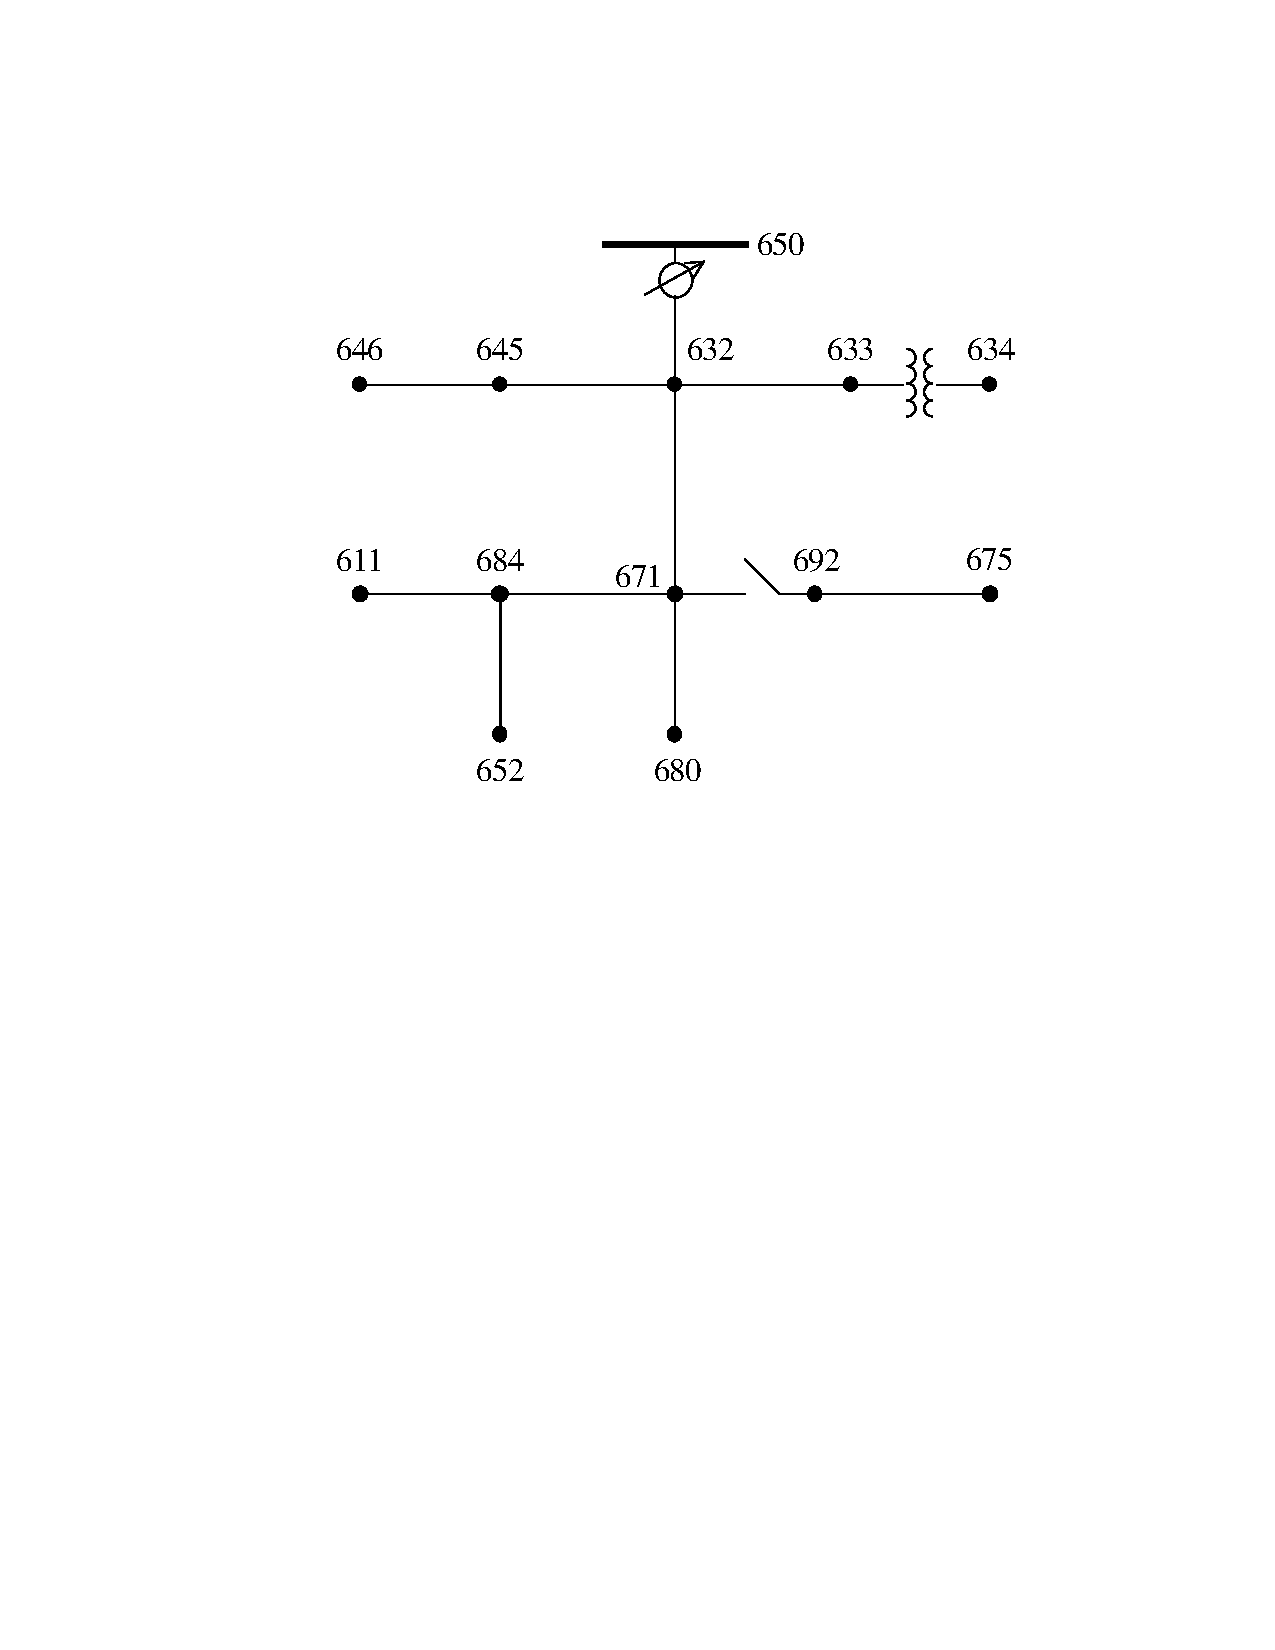
\includegraphics[width=3.0in]{13_node_feeder.pdf}
\caption{IEEE 13 node feeder model.}
\label{fig:13node}
\end{figure}

Feeder configurations, per-length line segment impedances, and line segment lengths can be found in \cite{IEEEtestfeeder}.  All line segment impedances were increased by a factor of 1.25. Spot loads (also found in \cite{IEEEtestfeeder}) were assigned to nodes according to Table \ref{tab:loads}. Distributed loads were neglected.  For the simulation, feeder power and voltage base values were chosen as the power rating and secondary voltage of the substation transformer, 500kVA and 4.16kV respectively.  Additionally, feeder head voltage was fixed to 1 p.u..  Controllable three phase inverter resources were placed at nodes 632, 675, 680, and 684.  These resources were purposefully left unconstrained to test the effectiveness of the OPF, with the ability to source or sink arbitrary amounts of reactive power. 

\begin{table}[h]
	\caption{SPOT LOADS OF 13 NODE FEEDER.}	
	\begin{center}
		\begin{tabular}{| l | c | c | c |}
        	\hline
        	& \multicolumn{3}{|c|}{Phase } \\
        	\hline
        	Node & $a$ [pu] & $b$ [pu] & $c$ [pu] \\
            \hline
			650 & 0 & 0 & 0 \\
            \hline
            632 & 0 & 0 & 0 \\
            \hline
            633 & 0 & 0 & 0 \\
            \hline
            634 & 0.032 + j 0.022 & 0.024 + j 0.018 & 0.024 + j 0.018 \\
            \hline
            645 & -- & 0.034 + j 0.025 & 0 \\
            \hline
            646 & -- & 0.046 + j 0.0264 & 0 \\
            \hline
            671 & 0.077 + j 0.044 & 0.077 + j 0.044 & 0.077 + j 0.044 \\
            \hline
            692 & 0 & 0 & 0.034 + j 0.0302 \\
            \hline
            675 & 0.097 + j 0.038 & 0.0136 + j 0.012 & 0.058 + j 0.0424 \\
            \hline
            680 & 0 & 0 & 0 \\
            \hline
            684 & 0 & -- & 0 \\
            \hline
            652 & 0.0256 + j 0.0172 & -- & -- \\
            \hline
            611 & -- & -- & 0.034 + j 0.0106 \\
            \hline
            Total & 0.2316 + j 0.1212 & 0.1946 + j 0.1254 & 0.227 + j 0.1506 \\
            \hline
		\end{tabular}
	\end{center}	
	\label{tab:loads}
\end{table}

Simulation results are presented in Figs. \ref{fig:Vres} - \ref{fig:unode} and in Table \ref{tab:unode}.  Voltage profiles for the base scenario (where inverter VAR resources are not utilized) and control scenario (inverter VAR resources are determined by the OPF of \eqref{eq:opt}) can be seen in Fig. \ref{fig:Vres}, with phase $a$, $b$ and $c$ voltage magnitudes plotted in Fig. \ref{fig:Va}, Fig. \ref{fig:Vb}, and Fig. \ref{fig:Vc}, respectively. As the figures show, in the control case, the voltage magnitudes of phase $a$ are kept almost constant with the base case. The voltage magnitudes of phase $b$ are decreased, and of $c$ are increased, to achieve greater voltage magnitude balance. Additionally, the voltages of phase $c$, originally in violation of the lower voltage bound, are now within the acceptable $\pm 5\%$ threshold.  It should be noted that the rise in voltage magnitude for the base scenario from node 632 to node 671 reconciles with power-flow simulation results in \cite{IEEEtestfeeder} and is likely due to the fact that off diagonal components of \eqref{eq:M}-\eqref{eq:N} have \emph{opposite} signs of the diagonal components, indicating that large voltage drops in some phases actually contribute to voltage \emph{rises} in other phases.

% As the figures show, in the control case the voltage magnitudes of phases $a$ and $c$ are increased compared to the base case, whereas the magnitudes of phase $b$ are decreased.  Additionally, the voltages of phase $c$, originally in violation of the lower voltage bound, are now within the acceptable $\pm 5\%$ threshold.

A comparison of voltage magnitudes for all phases at each node can be seen in Fig. \ref{fig:VbaseVcon}, with the base scenario in Fig. \ref{fig:Vbase}, and the control scenario in Fig. \ref{fig:Vcon}.  As the figures show, the voltage magnitudes are much closer together when inverter reactive power is dispatched according to the results of the OPF of \eqref{eq:opt}.

Figure \ref{fig:Vbalance} evaluates the first term of objective function of \eqref{eq:opt} for all nodes with and without control action.  The results show that the objective function value (which measures the Euclidian distance between squared voltage magnitudes) decreases at all nodes following control action with the exception of node 646, which increases very slightly.  

Optimal inverter control output is shown in Fig. \ref{fig:unode} and listed in \ref{tab:unode}.  As the figure shows, to balance the system, inverters at node 675 and 632 actually \emph{consume} VARs.  We believe that this effect occurs as these phase voltages are increasing compared to voltages in the remaining phases.

\begin{table}[h]
	\caption{OPTIMAL INVERTER VAR DISPATCH.}	
	\begin{center}
		\begin{tabular}{| l | c | c | c |}
        	\hline
        	& \multicolumn{3}{|c|}{Phase } \\
        	\hline
        	Node & $a$ [pu] & $b$ [pu] & $c$ [pu] \\
            \hline
% 			650 & 0 & 0 & 0 \\
%             \hline
            632 & -0.0081 & -0.0346 & 0.0437 \\
            \hline
%             633 & 0 & 0 & 0 \\
%             \hline
%             634 & 0 & 0 + j 0 \\
%             \hline
%             645 & 0 & 0 & 0 \\
%             \hline
%             646 & 0 & 0 & 0 \\
%             \hline
%             671 & 0 & 0 & 0 \\
%             \hline
%             692 & 0 & 0 & 0 \\
%             \hline
            675 & 0.005 & 0.0522 & -0.058 \\
            \hline
            680 & 0.003 & 0.0011 & -0.0038 \\
            \hline
            684 & -0.0003 & -- & -0.0389 \\
            \hline
%             652 & 0 & 0 & 0 \\
%             \hline
%             611 & 0 & 0 & 0 \\
%             \hline
            Total & -0.0003 & 0.0187 & -0.057 \\
            \hline
		\end{tabular}
	\end{center}	
	\label{tab:unode}
\end{table}

% We define a metric of voltage magnitude imbalance at a node as the Euclidean norm of all possible voltage magnitude differences at the node, as in \eqref{eq:imbal}. The imbalance for the base and control scenarios are shown in Fig. \ref{fig:Vbalance}.

% The total imbalance of the feeder is given by $\sum_{k \in H} J_{k}$, with a base scenario value of 0.3352 and control scenario value of 0.0283.

% \begin{equation}
% 	J_{k} = \left[ \sum_{ \substack{ {\phi, \psi \in \Phi_{i}} \\ {\phi \neq \psi} }} \left( \left| V_{\phi,k} \right| - \left| V_{\psi,k} \right| \right)^2 \right]^{1/2}
%     \label{eq:imbal}
% \end{equation}

% \begin{table}[!htb]
% 	\caption{COMPARISON OF FEEDER HEAD POWER FOR BASE AND CONTROL SCENARIOS.}	
% 	\begin{center}
% 		\begin{tabular}{| l c | c | c |}
%         	\hline
%         	& & Base scenario [pu] & Control Scenario [pu] \\
%             \hline
% 			Apparent Power & $S_{0}$ & 0.7842 & 0.7648 \\
%             \hline
%             Real Power & $P_{0}$ & 0.6588 & 0.6584 \\
%             \hline
%             Reactive Power & $Q_{0}$ & 0.4243 & 0.3824 \\
%             \hline
% 		\end{tabular}
% 	\end{center}	
% 	\label{tab:pow}
% \end{table}

% \begin{table}[!htb]
% 	\caption{DER CONTROL INPUTS.}	
% 	\begin{center}
% 		\begin{tabular}{| l | c | c | c |}
%         	\hline
%         	& \multicolumn{3}{|c|}{Phase } \\
%         	\hline
%         	Node & $a$ [VAr pu] & $b$ [VAr pu] & $c$ [VAr pu] \\
%             \hline
% 			632 & & & \\
%             \hline
%             675 & & &  \\
%             \hline
%             680 & & &  \\
%             \hline
%             684 & & & \\
%             \hline
% 		\end{tabular}
% 	\end{center}	
% 	\label{tab:uk}
% \end{table}

\begin{figure}[t]
\centering
\begin{subfigure}[b]{0.49\textwidth}
	\centering
	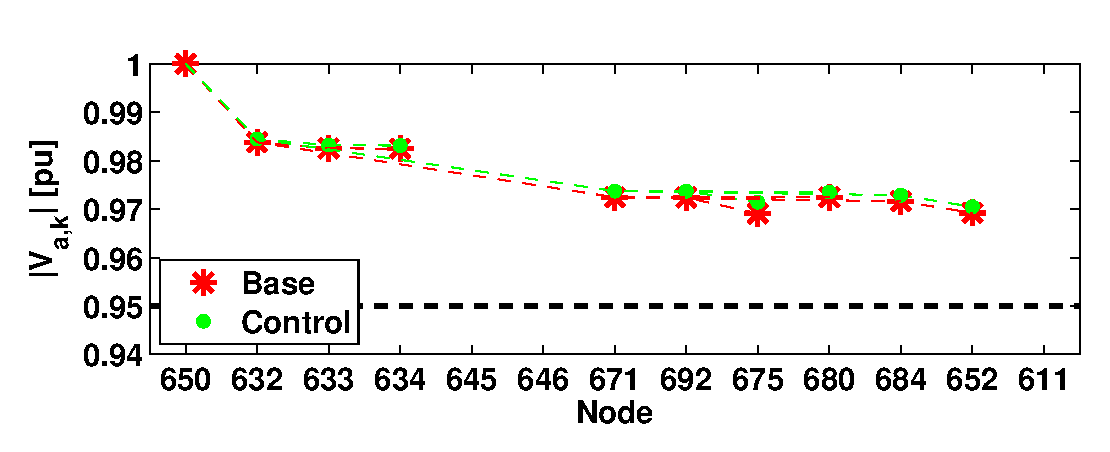
\includegraphics[width=\textwidth]{Va.eps}
	\caption{Phase $a$ voltage magnitudes.}
	\label{fig:Va}
\end{subfigure}
\\
\begin{subfigure}[b]{0.49\textwidth}
	\centering
	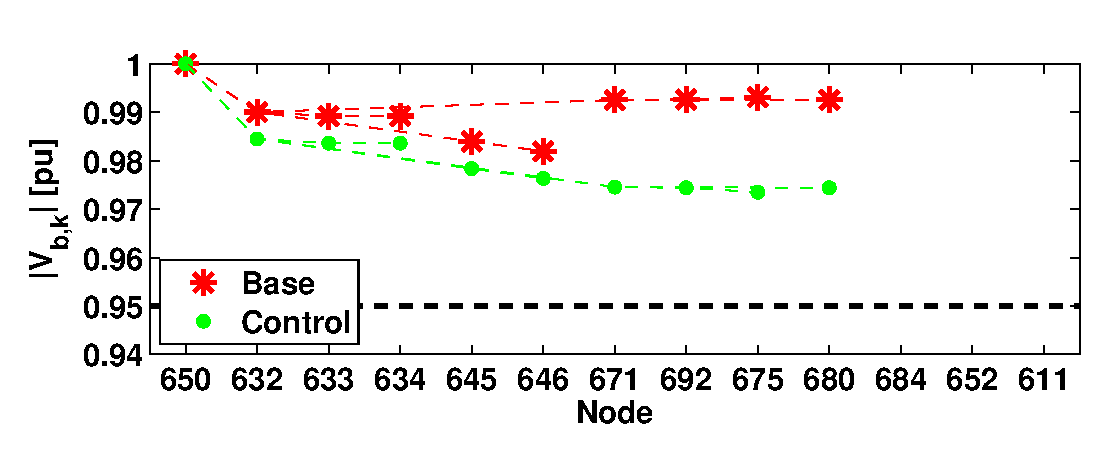
\includegraphics[width=\textwidth]{Vb.eps}
	\caption{Phase $b$ voltage magnitudes.}
	\label{fig:Vb}
\end{subfigure}
\\
\begin{subfigure}[b]{0.49\textwidth}
	\centering
	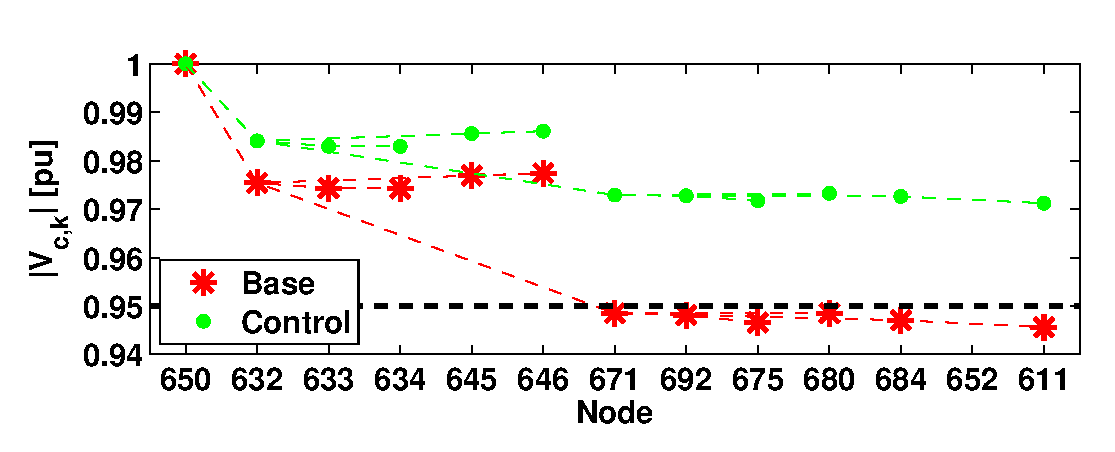
\includegraphics[width=\textwidth]{Vc.eps}
	\caption{Phase $c$ voltage magnitudes.}
	\label{fig:Vc}
\end{subfigure}
\caption{Phase $a$, $b$, and $c$ voltages magnitudes for base and control scenarios plotted individually. Dashed lines represent line segments between nodes.}
\label{fig:Vres}
\end{figure}

% \begin{figure}[t]
% 	\centering
% 	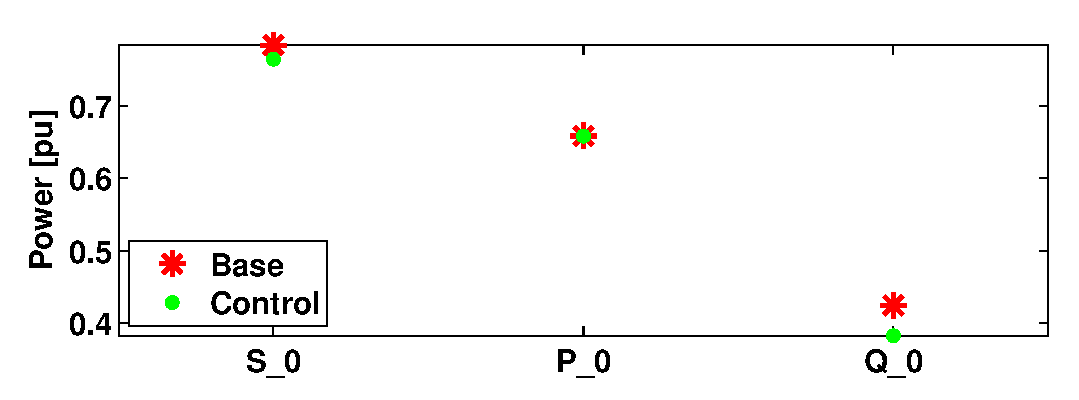
\includegraphics[width=0.5\textwidth]{SPQ.eps}
% 	\caption{Feeder head apparent, real and reactive power for the base and control scenarios.}
% 	\label{fig:SPQ}
% \end{figure}

\begin{figure*}[t]
	\centering
	\begin{subfigure}[b]{0.49\textwidth}
		\centering
		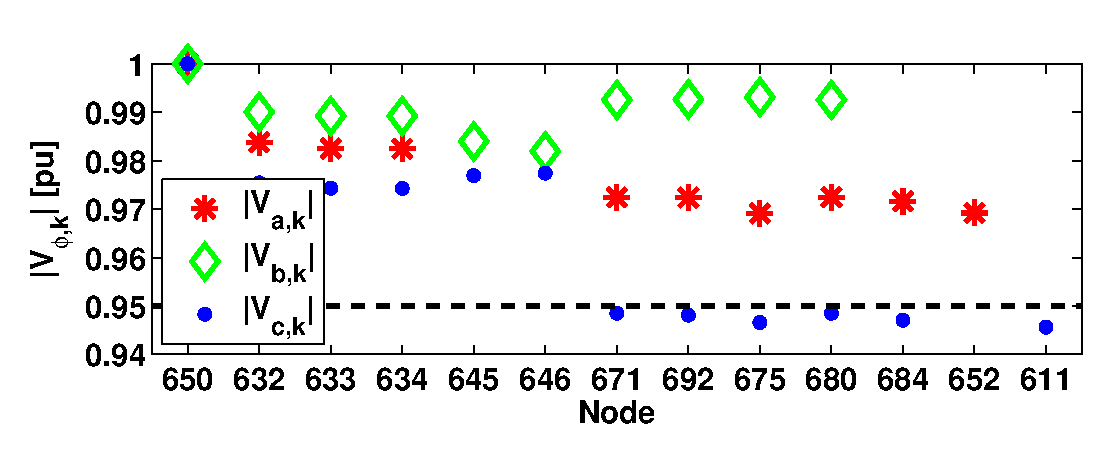
\includegraphics[width=\textwidth]{Vbase.eps}
		\caption{Voltage magnitudes without control.}
		\label{fig:Vbase}
	\end{subfigure}
    \begin{subfigure}[b]{0.49\textwidth}
		\centering
		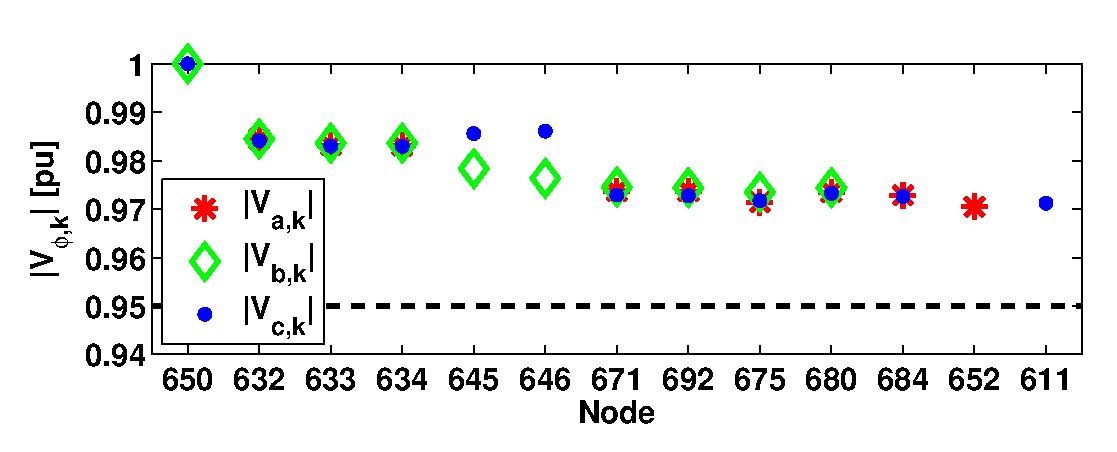
\includegraphics[width=\textwidth]{Vcon.eps}
		\caption{Voltage magnitudes with control.}
		\label{fig:Vcon}
	\end{subfigure}
    \caption{Phase $a$, $b$, and $c$ voltages magnitudes plotted together for base and control scenarios.}
	\label{fig:VbaseVcon}
\end{figure*}

\begin{figure}[t]
	\centering
	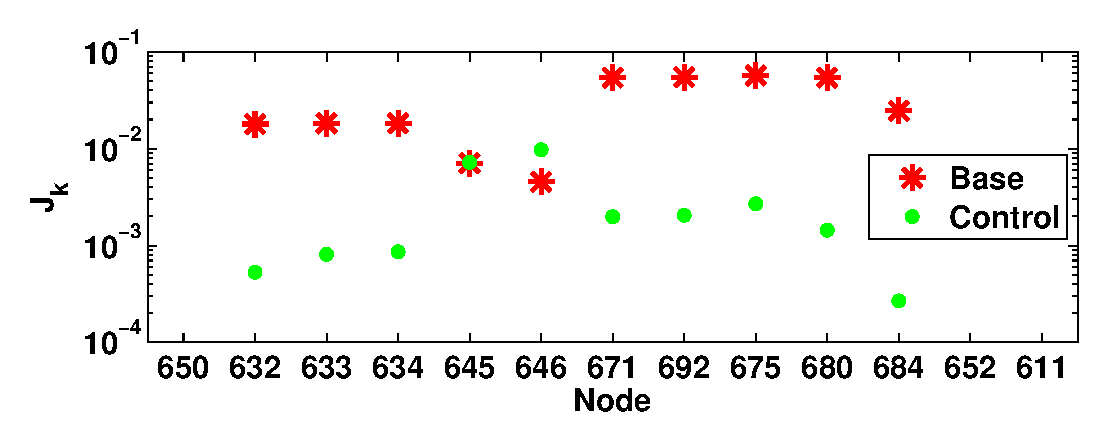
\includegraphics[width=0.5\textwidth]{Vbalance.eps}
	\caption{Phase voltage imbalance for all nodes, as defined in \eqref{eq:opt}.}
	\label{fig:Vbalance}
\end{figure}

\begin{figure}[t]
	\centering
	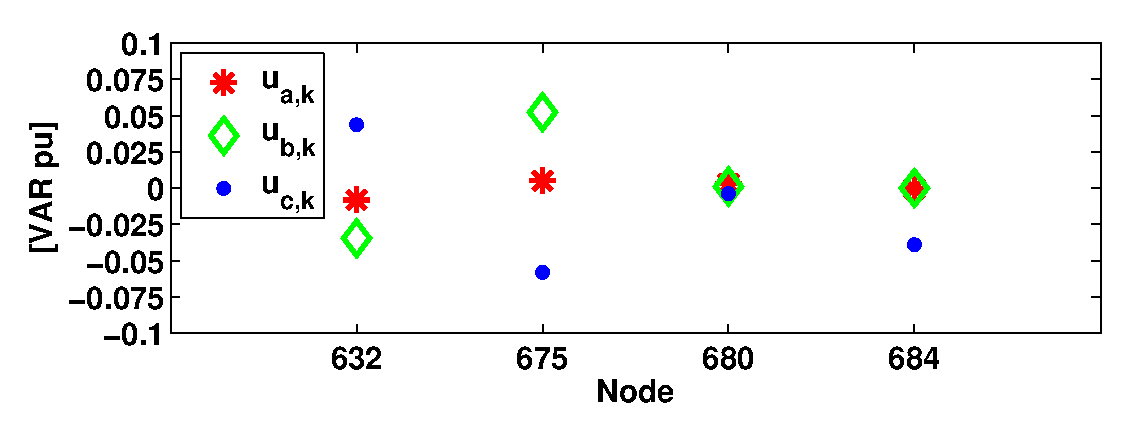
\includegraphics[width=0.5\textwidth]{unode.eps}
	\caption{Optimal inverter VAR resource.}
	\label{fig:unode}
\end{figure}

% \input{sim_sdpcomp}

% \input{sim_tracking}

\section{Conclusion}
\label{sec:conclusion}

Optimization of unbalanced power flow is a challenging topic due to its nonlinear and non-convex nature. While recent works on SDP relaxations  \cite{dall2012optimization} - \cite{dall2013distributed} have made OPF formulations for unbalanced systems possible, these approaches suffer from restrictions on the possible objectives and a high-dimensional geometrical complexity that impedes feasibility and uniqueness of the solutions.  In an effort to solve problems that cannot be addressed via SDP techniques, in this paper we sought to extend our previous work \cite{arnold2015optimal}, \cite{sankur2016linear} in developing an approximate model for distribution power flow that could be subsequently incorporated into optimal power flow problems.  

To do so, in Section \ref{sec:analysis} we developed a model that maps complex power flows into voltage angle differences.  It was noted that the complex power/voltage angle relationship shared a similar structure to the complex power/voltage magnitude relationship, in that they incorporated the imaginary part and real part, respectively, of the same vector of complex power flows. Due to this structure, we were able to utilize the linearizing assumptions in our previous efforts to simplify the voltage angle/complex power relationship, thereby extending the \emph{LinDist3Flow} system. The extended \emph{LinDist3Flow} model, henceforth, allowed the formulation of OPF problems that managed the entire voltage phasor, rather than only voltage magnitudes.  

Using this linear model, in Section \ref{sec:simulation_results}, we proposed an OPF to manage DER assets to enable ``clean'' switching in distribution systems (whereby minimal amounts of power flows through the switch after it is closed).  To accomplish this, the OPF sought to minimize the voltage phasor difference across a switch that separated a large islanded load and the distribution system.  The voltage phasor of the islanded load, which was assumed to be uncontrolled, was treated as a reference signal. The OPF then dispatched DER resources so that the voltage phasor on the feeder-side of the open switch was driven to this reference, while simultaneously maintaining proper voltage profiles in the rest of the system.  Simulation results showed the effectiveness of the OPF in driving the selected voltage phasor to meet the target.  In so doing, we ensured that, upon closing the switch, minimal amounts of power would flow across the switch resulting in a negligible disturbance in the feeder voltage profile. 

The ability to switch components into and out of distribution feeders with minimal impact on system operation presents many opportunities to reconfigure distribution systems for a variety of purposes.  Moving forward, we intend to investigate two such applications.  First, we plan to study grid reconfiguration in order to better withstand critical grid events (e.g. weather-related or other types of disasters).  In anticipation of a critical event, it may be advantageous to alter system topology to maximize the ability to serve critical loads.  To solve such a problem, we will most likely need to extend our present OPF formulation into a receding horizon controller, that can optimize over a future time window.  Secondly, as ``clean'' switching may also enable distributed microgrids to coalesce and pool resources to provide ancillary services, we intend to extend this OPF formulation to allow for mixed-integer formulations.  

% To do so, we derived a generalized model of distribution system power flow that maps real and reactive power injections into squared voltage magnitude differences.  The resulting model, which we referred to as the \textit{Dist3Flow} equations, can be viewed as an extension of the \textit{DistFlow} \cite{baran1989optimal} equations to 3-phase unbalanced distribution systems.  As the \textit{Dist3Flow} model is nonlinear and not necessarily convex, we suggested two procedures to linearize the system into a form suitable for incorporation into OPF formulations.  The linearized power flow model, which we have referred to as the \textit{LinDist3Flow} system, is obtained by approximating the nonlinear components of the original equations.  

% The first approximation procedure treated the ratio of voltages of different phases as a constant and neglected line losses.  The resulting \textit{LinDist3Flow} system was tested in an OPF with the objective of minimizing feeder-head real power.  Comparison of results obtained to a SDP formulation of the same problem revealed that the OPF driven by the \emph{LinDist3Flow} model achieved a solution whose objective function was within 0.2\% of the optimal value.
% The second procedure for approximating the \textit{Dist3Flow} equations involved iterating over the nonlinear terms between successive runs of solving the power flow equations and then solving the OPF.  This approach was simulated in an OPF formulation with the objective of regulating and balancing system voltages, and was shown to increase accuracy compared to the previous approximation technique. 

%  Although it is an approximation, the principle advantage of \emph{LinDist3Flow} model is that it enables an optimal power flow schemes where the constraints are linear and convex relaxations are not required.  As such, for strictly convex objectives with a non-empty feasible  set, the OPF will always find an optimal solution to the approximate problem.  As was mentioned previously, an OPF driven by the \textit{LinDist3Flow} model was able to solve a voltage balancing optimization, for which, by the knowledge of the authors, a SDP formulation does not exist.  Although the final solution is only approximate. The iterative method shows potential for further improving the accuracy gap between the linear and full nonlinear model, and future work will consider mathematical analysis to characterize this.

% The feasibility of the \emph{LinDist3Flow} model can be exploited in OPF formulations with a variety of relevant objectives, such as voltage balancing, loss minimization, or economic dispatch. Our future work is aimed at exploring other useful applications of three phase unbalanced OPF such as voltage reference tracking or battery and electric vehicle charging. First, we will use our findings to extend the authors' work on optimal decentralized voltage regulation  \cite{sondermeijer2015regression}, developed for single-phase balanced networks, to 3-phase unbalanced systems. Furthermore, in a recent work, the authors developed a framework for distribution grid state estimation with limited sensing and forecasting information, using linearized power flow equations for single-phase systems \cite{dobbe2015real}. We aim to extend these results to unbalanced systems using the \emph{LinDist3Flow} equations.


\section*{Appendix}
\label{sec:appendix}

\emph{Extension of Semidefinite OPF of \cite{dall2012optimization}, \cite{dall2013distributed}: } We start by rewriting the matrix variable $X = v {v}^{*}$, where $v = {\left[ \mathbb{V}_{0}^{T}, \text{ } \mathbb{V}_{1}^{T}, \text{ } \ldots \text{ } \mathbb{V}_{N}^{T} \right]}^{T}$ and $\mathbb{V}_{n} = {\left[ V_{n}^{a}, \text{ } V_{n}^{b}, \textbf{ } V_{n}^{c} \right]}^{T}$. Consider a reference magnitude for phase $\phi$ at node $n$, $\Upsilon_{n}^{\phi}$; Adding the following equality constraint to the OPF formulation will ensure  $\left| V_{n}^{\phi} \right| = \Upsilon_{n}^{\phi}$, as $\left| V_{n}^{\phi} \right| = \Upsilon_{n}^{\phi} \Rightarrow \left| V_{n}^{\phi} \right|^{2} = {\left( \Upsilon_{n}^{\phi} \right)}^{2} \Rightarrow V_{n}^{\phi} {\left( V_{n}^{\phi} \right)}^{*} = {\left( \Upsilon_{n}^{\phi} \right)}^{2}$:
\begin{equation}
	\Tr \left( \Phi_{V,n}^{\phi} X \right) = {\left( \Upsilon_{n}^{\phi} \right)}^{2}
\end{equation}

\noindent where $\Phi_{V,n}^{\phi} = e_{n}^{\phi} {\left( e_{n}^{\phi} \right)}^{T}$ as in \cite{dall2012optimization}.

Now, consider an off-diagonal entry of $X$, $X_{n0}^{\phi} = V_{n}^{\phi} {\left( V_{0}^{\phi} \right)}^{*}$, corresponding to the product of the phasor of phase $\phi$ at node $n$, and the complex conjugate of the phasor of phase $\phi$ at node 0. Here, we express this term in polar form:
% \begin{align}
% 	V_{n}^{\phi} \left( V_{0}^{\phi} \right)^{*}
%     &= \left| V_{n}^{\phi} \right| \left| V_{0}^{\phi} \right| \angle \left( \theta_{n}^{\phi} - \theta_{0}^{\phi} \right) \label{VnV0polar} \\
%     &= \left| V_{n}^{\phi} \right| \left| V_{0}^{\phi} \right| \exp \left( j \left( \theta_{n}^{\phi} - \theta_{0}^{\phi} \right) \right) \label{VnV0rect}
%     V_{n}^{\phi} \left( V_{0}^{\phi} \right)^{*}
%     &= \left| V_{n}^{\phi} \right| \left| V_{0}^{\phi} \right| \left[ \cos \left( \theta_{n}^{\phi} - \theta_{0}^{\phi} \right) + j \sin \left( \theta_{n}^{\phi} - \theta_{0}^{\phi} \right) \right] \label{VnV0rect} 
% \end{align}
\begin{equation}
	X_{n0}^{\phi} = V_{n}^{\phi} {\left( V_{0}^{\phi} \right)}^{*} = \left| V_{n}^{\phi} \right| \left| V_{0}^{\phi} \right| \angle \left( \theta_{n}^{\phi} - \theta_{0}^{\phi} \right) \label{VnV0polar}
\end{equation}

% \begin{equation}
% 	V_{n}^{\phi} \left( V_{0}^{\phi} \right)^{*} = \left| V_{n}^{\phi} \right| \left| V_{0}^{\phi} \right| \left[ \cos \left( \theta_{n}^{\phi} - \theta_{0}^{\phi} \right) + j \sin \left( \theta_{n}^{\phi} - \theta_{0}^{\phi} \right) \right] \label{VnV0rect} 
% \end{equation}

\noindent Using Euler's rule, we write the the real and imaginary parts of $X_{0n}^{\phi}$ in terms of the tangent of $\theta_{n}^{\phi} - \theta_{0}^{\phi}$:
% \begin{equation}
% 	\tan \left( \theta_{n}^{\phi} - \theta_{0}^{\phi} \right)
% %     =
% %     \frac{\sin \left( \theta_{n}^{\phi} - \theta_{0}^{\phi} \right)}{\cos \left( \theta_{n}^{\phi} - \theta_{0}^{\phi} \right)}
%     =
%     \frac{\Im \left\{ V_{n}^{\phi} \left( V_{0}^{\phi} \right)^{*} \right\}}{\Re \left\{ V_{n}^{\phi} \left( V_{0}^{\phi} \right)^{*} \right\}}.
%     \label{eq:tanVkV0}
% \end{equation}
\begin{equation}
	\Re \left\{ V_{n}^{\phi} {\left( V_{0}^{\phi} \right)}^{*} \right\} \tan \left( \theta_{n}^{\phi} - \theta_{0}^{\phi} \right)
    =
    \Im \left\{ V_{n}^{\phi} {\left( V_{0}^{\phi} \right)}^{*} \right\}
\end{equation}

\noindent The real and imaginary parts of $V_{n}^{\phi} \left( V_{0}^{\phi} \right)^{*}$ are defined as:
\begin{align}
	\Re \left\{ V_{n}^{\phi} \left( V_{0}^{\phi} \right)^{*} \right\}
    &= 
    \frac{1}{2} \left[ V_{n}^{\phi} {\left( V_{0}^{\phi} \right)}^{*} + V_{0}^{\phi} {\left( V_{n}^{\phi} \right)}^{*} \right] \nonumber \\
    &=
    \frac{1}{2} \left[ \Tr \left( \Phi_{V,n0}^{\phi} X \right) + \Tr \left( \Phi_{V,0n}^{\phi} X \right) \right] \\
    \Im \left\{ V_{n}^{\phi} \left( V_{0}^{\phi} \right)^{*} \right\}
    &=
    \frac{1}{j2} \left[ V_{n}^{\phi} {\left( V_{0}^{\phi} \right)}^{*} - V_{0}^{\phi} {\left( V_{n}^{\phi} \right)}^{*} \right] \nonumber \\
    &=
    \frac{1}{j2} \left[ \Tr \left( \Phi_{V,n0}^{\phi} X \right) - \Tr \left( \Phi_{V,0n}^{\phi} X \right) \right],
\end{align}

\noindent where $\Phi_{V,n0}^{\phi} = e_{0}^{\phi} {\left( e_{n}^{\phi} \right)}^{T}$ and $\Phi_{V,0n}^{\phi} = e_{n}^{\phi} {\left( e_{0}^{\phi} \right)}^{T}$ using the same convention for $e_{n}^{\phi}$ as in \cite{dall2012optimization}. With some matrix algebra, we obtain equality constraints for the phase angle:
% \begin{align*}
% 	& \Tr \left( \left( \Phi_{n0}^{\phi} + \Phi_{0n}^{\phi} \right) X \right)
%     \tan \left( \theta_{n}^{\phi} - \theta_{0}^{\phi} \right) = \ldots \nonumber \\
%     & \quad -j \Tr \left( \left( \Phi_{n0}^{\phi} - \Phi_{0n}^{\phi} \right) X \right),
% \end{align*}
% \noindent which can be restated:
\begin{align}
     & \Tr \left(\Phi_{\theta,n}^{\phi} X \right) = 0 \label{eq:SDPangeq} \\
     & \Phi_{\theta,n}^{\phi} = \tan \left( \theta_{n}^{\phi} - \theta_{0}^{\phi} \right)
    \left( \Phi_{V,n0}^{\phi} + \Phi_{V,0n}^{\phi} \right)
    \nonumber \\
     & \quad +
    j \left( \Phi_{V,n0}^{\phi} - \Phi_{V,0n}^{\phi} \right).
    \label{eq:PhiVn0}
\end{align}

In this derivation we reference the phase angle of phase $\phi$ at node $n$ to that of phase $\phi$ at node $0$. This formulation is easily modified to reference phase angles to a common or arbitrary reference.

The nature of SDPs disallows incorporation of the L2 norm, thus we were unable to formulate \eqref{eq:OPF} as an SDP. However, it is possible to formulate the SDP with an L1 norm minimization. We write an example objective function for an OPF where one node has a voltage magnitude reference:
\begin{equation}
	\min_{X} \sum_{\phi \in \{ a,b,c \}} \left| \Tr \left( \Phi_{V,n}^{\phi} X \right) - \Upsilon_{n}^{\phi} \right|
\end{equation}

\noindent This can be extended to a problem with multiple nodes having magnitude references. Similarly, \eqref{eq:SDPangeq} and \eqref{eq:PhiVn0} can be used in the same manner for phase angle references.

% \section{SDP Method}

We use the same notation as in \cite{dall2012optimization} where $\mathbb{V}_{n} \in \mathbb{C}^{3 \times 1}$ denotes a vector of three voltage phasors in $\left\{ a,b,c \right\}$ order:
\begin{equation}
	V_{n} = 
    \begin{bmatrix}
    	\mathbb{V}_{n}^{a} & V_{n}^{b} & V_{n}^{c}
    \end{bmatrix}^{T}.
\end{equation}

\noindent The vector $v$ collects all $V_{n}, \text{ } n \in \mathcal{N}$:
\begin{equation}
    v = 
    \begin{bmatrix}
    	\mathbb{V}_{0}^{T} & \mathbb{V}_{1}^{T} & \hdots & \mathbb{V}_{N}^{T}
    \end{bmatrix}^{T},
\end{equation}

\noindent and the matrix variable $X$ is defined as:
\begin{equation}
    X = v v^{*}
\end{equation}
\begin{equation}
    X =
    \begin{bmatrix}
    	\mathbb{V}_{0} \left( \mathbb{V}_{0} \right)^{*} & \mathbb{V}_{0} \left( \mathbb{V}_{1} \right)^{*} & \hdots & \mathbb{V}_{0} \left( \mathbb{V}_{N} \right)^{*} \\
        \mathbb{V}_{1} \left( \mathbb{V}_{0} \right)^{*} & \mathbb{V}_{1} \left( \mathbb{V}_{1} \right)^{*} & \hdots & \mathbb{V}_{1} \left( \mathbb{V}_{N} \right)^{*} \\
        \vdots & \vdots & \ddots & \vdots \\
        \mathbb{V}_{N} \left( \mathbb{V}_{0} \right)^{*} & \mathbb{V}_{N} \left( \mathbb{V}_{1} \right)^{*} & \hdots & \mathbb{V}_{N} \left( \mathbb{V}_{N} \right)^{*}
    \end{bmatrix}
\end{equation}

\noindent where the ${}^{*}$ superscript denotes the complex conjugate of a scalar or matrix. The feeder head voltage is fixed as
% $V_{0} = \begin{bmatrix} 1 & \alpha^{*} & \alpha \end{bmatrix}^{T}$
$\mathbb{V}_{0} = \begin{bmatrix} V_{0}^{a} & V_{0}^{b} & V_{0}^{c} \end{bmatrix}^{T}$
such that the block of $X$ corresponding to node $0$ is:
\begin{equation}
    X(1:3,1:3) = X_{00} = 
%     \begin{bmatrix}
%     	1 & \alpha & \alpha^* \\
%         \alpha^* & 1 & \alpha \\
%         \alpha & \alpha^* & 1
%     \end{bmatrix}
	\mathbb{V}_{0} \left( \mathbb{V}_{0}  \right)^{*}.
\end{equation}

\subsection{Magnitude}

\subsubsection{Constraint}

Here, we provide an extension of the work in \cite{dall2012optimization} to include a method for enforcing one or more voltage phasor magnitudes.

\begin{equation}
	\left| V_{n}^{\phi} \right| = r_{n}^{\phi} \Rightarrow V_{n}^{\phi} \left( V_{n}^{\phi} \right) ^{*} = \left( r_{n}^{\phi} \right)^{2} \Rightarrow \Tr \left( \Phi_{V,n}^{\phi} X \right) = \left( r_{n}^{\phi} \right)^{2}
\end{equation}

\subsubsection{Tracking}

This is how we would do the SDP Magnitude formulation with 1 norm minimization, if it worked \\

Augment SDP variable with real valued matrix $\Gamma$
\begin{equation}
	X^{'} = v v^{*},
    \quad
    X =
    \begin{bmatrix}
    	X^{'} & 0 \\
        0 & \Gamma
    \end{bmatrix}
\end{equation}

Define $\Gamma$ matrix and diagonal block matrices corresponding to nodes
\begin{equation}
    \Gamma = 
%     \begin{bmatrix}
%     	\gamma_{1}^{a} & 0 & 0 \\
%         0 & \gamma_{1}^{b} & 0 \\
%         0 & 0 & \gamma_{1}^{c} \\
%         asdf \\
%         0 & 0 & 0 & \hdots &\gamma_{N}^{c}
%     \end{bmatrix}
    \begin{bmatrix}
    	\Gamma_{0} & 0 & \hdots & 0 \\
        0 & \Gamma_{1} & \hdots & 0 \\
        \vdots & \vdots & \ddots & 0 \\
        0 & 0 & \hdots &\Gamma_{N}
    \end{bmatrix},
    \quad
    \Gamma_{n} = 
    \begin{bmatrix}
    	\gamma_{n}^{a} & 0 & 0 \\
        0 & \gamma_{n}^{b} & 0 \\
        0 & 0 & \gamma_{n}^{c}
    \end{bmatrix}
\end{equation}

Define magnitude 1 norm for objective function and how to put into a linear constraint
\begin{equation}
	\left| V_{n}^{\phi} \left( V_{n}^{\phi} \right)^{*} - \left( r_{n}^{\phi} \right)^{2} \right|
    =
	\left| \left| V_{n}^{\phi} \right|^{2} - \left( r_{n}^{\phi} \right)^{2} \right| \leq \gamma_{n}^{\phi}
\end{equation}

Linear version of previous eq
\begin{align}
	\left| V_{n}^{\phi} \right|^{2} - \left( r_{n}^{\phi} \right)^{2} & \leq \gamma_{n}^{\phi} \\
    - \left( \left| V_{n}^{\phi} \right|^{2} - \left( r_{n}^{\phi} \right)^{2} \right) & \leq \gamma_{n}^{\phi}
\end{align}

Trace constraints, update to use large X instead of X and Gamma
\begin{align}
	\Tr \left( \Phi_{V,n}^{\phi} X \right) - \left( r_{n}^{\phi} \right)^{2} & \leq \Tr \left( \Phi_{\Gamma,n}^{\phi} \Gamma \right) \\
    - \left( \Tr \left( \Phi_{V,n}^{\phi} X \right) - \left( r_{n}^{\phi} \right)^{2} \right) & \leq \Tr \left( \Phi_{\Gamma,n}^{\phi} \Gamma \right)
\end{align}

\subsection{Angle}

We consider an off-diagonal entry of $X$, $X_{0n}^{\phi} = V_{n}^{\phi} \left( V_{0}^{\phi} \right)^{*}$, corresponding to the product of the phasor of phase $\phi$ at node $n$, and the complex conjugate of the phasor of phase $\phi$ at node 0. Here, we write out this term in polar \eqref{VnV0polar} and rectangular \eqref{VnV0rect} forms.
\begin{align}
	V_{n}^{\phi} \left( V_{0}^{\phi} \right)^{*} &= \left| V_{n}^{\phi} \right| \left| V_{0}^{\phi} \right| \angle \left( \theta_{n}^{\phi} - \theta_{0}^{\phi} \right) \label{VnV0polar} \\
%     &= \left| V_{n}^{\phi} \right| \left| V_{0}^{\phi} \right| \left[ \cos \left( \theta_{n}^{\phi} - \theta_{0}^{\phi} \right) + j \sin \left( \theta_{n}^{\phi} - \theta_{0}^{\phi} \right) \right] \label{VnV0rect}
    &= \left| V_{n}^{\phi} \right| \left| V_{0}^{\phi} \right| \exp \left( j \left( \theta_{n}^{\phi} - \theta_{0}^{\phi} \right) \right) \label{VnV0rect} 
\end{align}

\begin{equation}
	V_{n}^{\phi} \left( V_{0}^{\phi} \right)^{*} = \left| V_{n}^{\phi} \right| \left| V_{0}^{\phi} \right| \angle \left( \theta_{n}^{\phi} - \theta_{0}^{\phi} \right) \label{VnV0polar} \\
%     &= \left| V_{n}^{\phi} \right| \left| V_{0}^{\phi} \right| \left[ \cos \left( \theta_{n}^{\phi} - \theta_{0}^{\phi} \right) + j \sin \left( \theta_{n}^{\phi} - \theta_{0}^{\phi} \right) \right] \label{VnV0rect}
%     &= \left| V_{n}^{\phi} \right| \left| V_{0}^{\phi} \right| \exp \left( j \left( \theta_{n}^{\phi} - \theta_{0}^{\phi} \right) \right) \label{VnV0rect} 
\end{equation}

\begin{equation}
	V_{n}^{\phi} \left( V_{0}^{\phi} \right)^{*} = \left| V_{n}^{\phi} \right| \left| V_{0}^{\phi} \right| \left[ \cos \left( \theta_{n}^{\phi} - \theta_{0}^{\phi} \right) + j \sin \left( \theta_{n}^{\phi} - \theta_{0}^{\phi} \right) \right] \label{VnV0rect} 
\end{equation}

\noindent Using Euler's Rule, we can define the tangent of the angle difference, $ \Delta_{n}^{\phi} = \theta_{n}^{\phi} - \theta_{0}^{\phi}$, as the ratio of the real and imaginary parts of $X_{0n}^{\phi}$ is defined by the tangent of the angle difference:
\begin{equation}
	\tan \left( \theta_{n}^{\phi} - \theta_{0}^{\phi} \right)
    =
    \frac{\sin \left( \theta_{n}^{\phi} - \theta_{0}^{\phi} \right)}{\cos \left( \theta_{n}^{\phi} - \theta_{0}^{\phi} \right)}
    =
    \frac{\Im \left\{ V_{n}^{\phi} \left( V_{0}^{\phi} \right)^{*} \right\}}{\Re \left\{ V_{n}^{\phi} \left( V_{0}^{\phi} \right)^{*} \right\}}.
    \label{eq:tanVkV0}
\end{equation}

\noindent The real and imaginary parts of $V_{n}^{\phi} \left( V_{0}^{\phi} \right)^{*}$ are defined as:
\begin{align}
	\Re \left\{ V_{n}^{\phi} \left( V_{0}^{\phi} \right)^{*} \right\}
    &= 
    \frac{1}{2} \left[ V_{n}^{\phi} \left( V_{0}^{\phi} \right)^{*} + V_{0}^{\phi} \left( V_{n}^{\phi} \right)^{*} \right] \\
    &=
    \frac{1}{2} \left[ \Tr \left( \Phi_{n0}^{\phi} X \right) + \Tr \left( \Phi_{0n}^{\phi} X \right) \right] \label{eq:ReVkV0} \\
    \Im \left\{ V_{n}^{\phi} \left( V_{0}^{\phi} \right)^{*} \right\}
    &=
    \frac{1}{j2} \left[ V_{n}^{\phi} \left( V_{0}^{\phi} \right)^{*} - V_{0}^{\phi} \left( V_{n}^{\phi} \right)^{*} \right] \\
    &=
    \frac{1}{j2} \left[ \Tr \left( \Phi_{n0}^{\phi} X \right) - \Tr \left( \Phi_{0n}^{\phi} X \right) \right], \label{eq:ImVkV0}
\end{align}

\noindent where $\Phi_{n0}^{\phi}$ and $\Phi_{0n}^{\phi}$ are defined as in \eqref{eq:Phi}, using the same convention for $e_{n}^{\phi}$ as in \cite{dall2012optimization}:
\begin{equation}
	\Phi_{n0}^{\phi} = e_{0}^{\phi} \left( e_{n}^{\phi} \right)^{T},
    \quad
    \Phi_{0n}^{\phi} = e_{n}^{\phi} \left( e_{0}^{\phi} \right)^{T}.
    \label{eq:Phi}
\end{equation}

\noindent Thus, we can use \eqref{eq:tanVkV0} - \eqref{eq:Phi} to obtain equality constraints to be applied to be SDP:
% \begin{align}
% 	& \left[ \Tr \left( \Phi_{n0}^{\phi} X \right) + \Tr \left( \Phi_{0n}^{\phi} X \right) \right]
%     \tan \left( \theta_{n}^{\phi} - \theta_{0}^{\phi} \right)
%     = \ldots \\
%     & \quad -j \left[ \Tr \left( \Phi_{n0}^{\phi} X \right) - \Tr \left( \Phi_{0n}^{\phi} X \right) \right],
% \end{align}
% \begin{equation}
% 	\Tr \left( \left( \Phi_{n0}^{\phi} + \Phi_{0n}^{\phi} \right) X \right)
%     \tan \left( \theta_{n}^{\phi} - \theta_{0}^{\phi} \right)
%     =
%     -j \Tr \left( \left( \Phi_{n0}^{\phi} - \Phi_{0n}^{\phi} \right) X \right),
% \end{equation}
\begin{align}
	& \Tr \left( \left( \Phi_{n0}^{\phi} + \Phi_{0n}^{\phi} \right) X \right)
    \tan \left( \theta_{n}^{\phi} - \theta_{0}^{\phi} \right)
    = \ldots \nonumber \\
    & \quad -j \Tr \left( \left( \Phi_{n0}^{\phi} - \Phi_{0n}^{\phi} \right) X \right),
\end{align}

\noindent which can be restated:
\begin{align}
    & \Tr \left(\Phi_{\theta,n}^{\phi} X \right) = 0 \\
    & \Phi_{\theta,n}^{\phi} = \tan \left( \theta_{n}^{\phi} - \theta_{0}^{\phi} \right)
    \left( \Phi_{n0}^{\phi} + \Phi_{0n}^{\phi} \right)
    +
    j \left( \Phi_{n0}^{\phi} - \Phi_{0n}^{\phi} \right).
\end{align}

\noindent In this work we choose to reference the phase angle of a phase $\phi$ at node $n$ to the phase angle of phase $\phi$ at node $0$. This formulation can easily be modified to reference phase angles to a common or arbitrary reference. \\

%%%%%%%%%%%%%%%%%%%%%%%%%%%%%%%%%%%%%%%%%%%%%%%%%%
%% REFERENCES
%%%%%%%%%%%%%%%%%%%%%%%%%%%%%%%%%%%%%%%%%%%%%%%%%%

\bibliography{ref}
\bibliographystyle{IEEEtran}

\end{document}
